% Options for packages loaded elsewhere
\PassOptionsToPackage{unicode}{hyperref}
\PassOptionsToPackage{hyphens}{url}
%
\documentclass[
]{book}
\usepackage{amsmath,amssymb}
\usepackage{lmodern}
\usepackage{iftex}
\ifPDFTeX
  \usepackage[T1]{fontenc}
  \usepackage[utf8]{inputenc}
  \usepackage{textcomp} % provide euro and other symbols
\else % if luatex or xetex
  \usepackage{unicode-math}
  \defaultfontfeatures{Scale=MatchLowercase}
  \defaultfontfeatures[\rmfamily]{Ligatures=TeX,Scale=1}
\fi
% Use upquote if available, for straight quotes in verbatim environments
\IfFileExists{upquote.sty}{\usepackage{upquote}}{}
\IfFileExists{microtype.sty}{% use microtype if available
  \usepackage[]{microtype}
  \UseMicrotypeSet[protrusion]{basicmath} % disable protrusion for tt fonts
}{}
\makeatletter
\@ifundefined{KOMAClassName}{% if non-KOMA class
  \IfFileExists{parskip.sty}{%
    \usepackage{parskip}
  }{% else
    \setlength{\parindent}{0pt}
    \setlength{\parskip}{6pt plus 2pt minus 1pt}}
}{% if KOMA class
  \KOMAoptions{parskip=half}}
\makeatother
\usepackage{xcolor}
\usepackage{color}
\usepackage{fancyvrb}
\newcommand{\VerbBar}{|}
\newcommand{\VERB}{\Verb[commandchars=\\\{\}]}
\DefineVerbatimEnvironment{Highlighting}{Verbatim}{commandchars=\\\{\}}
% Add ',fontsize=\small' for more characters per line
\usepackage{framed}
\definecolor{shadecolor}{RGB}{248,248,248}
\newenvironment{Shaded}{\begin{snugshade}}{\end{snugshade}}
\newcommand{\AlertTok}[1]{\textcolor[rgb]{0.94,0.16,0.16}{#1}}
\newcommand{\AnnotationTok}[1]{\textcolor[rgb]{0.56,0.35,0.01}{\textbf{\textit{#1}}}}
\newcommand{\AttributeTok}[1]{\textcolor[rgb]{0.77,0.63,0.00}{#1}}
\newcommand{\BaseNTok}[1]{\textcolor[rgb]{0.00,0.00,0.81}{#1}}
\newcommand{\BuiltInTok}[1]{#1}
\newcommand{\CharTok}[1]{\textcolor[rgb]{0.31,0.60,0.02}{#1}}
\newcommand{\CommentTok}[1]{\textcolor[rgb]{0.56,0.35,0.01}{\textit{#1}}}
\newcommand{\CommentVarTok}[1]{\textcolor[rgb]{0.56,0.35,0.01}{\textbf{\textit{#1}}}}
\newcommand{\ConstantTok}[1]{\textcolor[rgb]{0.00,0.00,0.00}{#1}}
\newcommand{\ControlFlowTok}[1]{\textcolor[rgb]{0.13,0.29,0.53}{\textbf{#1}}}
\newcommand{\DataTypeTok}[1]{\textcolor[rgb]{0.13,0.29,0.53}{#1}}
\newcommand{\DecValTok}[1]{\textcolor[rgb]{0.00,0.00,0.81}{#1}}
\newcommand{\DocumentationTok}[1]{\textcolor[rgb]{0.56,0.35,0.01}{\textbf{\textit{#1}}}}
\newcommand{\ErrorTok}[1]{\textcolor[rgb]{0.64,0.00,0.00}{\textbf{#1}}}
\newcommand{\ExtensionTok}[1]{#1}
\newcommand{\FloatTok}[1]{\textcolor[rgb]{0.00,0.00,0.81}{#1}}
\newcommand{\FunctionTok}[1]{\textcolor[rgb]{0.00,0.00,0.00}{#1}}
\newcommand{\ImportTok}[1]{#1}
\newcommand{\InformationTok}[1]{\textcolor[rgb]{0.56,0.35,0.01}{\textbf{\textit{#1}}}}
\newcommand{\KeywordTok}[1]{\textcolor[rgb]{0.13,0.29,0.53}{\textbf{#1}}}
\newcommand{\NormalTok}[1]{#1}
\newcommand{\OperatorTok}[1]{\textcolor[rgb]{0.81,0.36,0.00}{\textbf{#1}}}
\newcommand{\OtherTok}[1]{\textcolor[rgb]{0.56,0.35,0.01}{#1}}
\newcommand{\PreprocessorTok}[1]{\textcolor[rgb]{0.56,0.35,0.01}{\textit{#1}}}
\newcommand{\RegionMarkerTok}[1]{#1}
\newcommand{\SpecialCharTok}[1]{\textcolor[rgb]{0.00,0.00,0.00}{#1}}
\newcommand{\SpecialStringTok}[1]{\textcolor[rgb]{0.31,0.60,0.02}{#1}}
\newcommand{\StringTok}[1]{\textcolor[rgb]{0.31,0.60,0.02}{#1}}
\newcommand{\VariableTok}[1]{\textcolor[rgb]{0.00,0.00,0.00}{#1}}
\newcommand{\VerbatimStringTok}[1]{\textcolor[rgb]{0.31,0.60,0.02}{#1}}
\newcommand{\WarningTok}[1]{\textcolor[rgb]{0.56,0.35,0.01}{\textbf{\textit{#1}}}}
\usepackage{longtable,booktabs,array}
\usepackage{calc} % for calculating minipage widths
% Correct order of tables after \paragraph or \subparagraph
\usepackage{etoolbox}
\makeatletter
\patchcmd\longtable{\par}{\if@noskipsec\mbox{}\fi\par}{}{}
\makeatother
% Allow footnotes in longtable head/foot
\IfFileExists{footnotehyper.sty}{\usepackage{footnotehyper}}{\usepackage{footnote}}
\makesavenoteenv{longtable}
\usepackage{graphicx}
\makeatletter
\def\maxwidth{\ifdim\Gin@nat@width>\linewidth\linewidth\else\Gin@nat@width\fi}
\def\maxheight{\ifdim\Gin@nat@height>\textheight\textheight\else\Gin@nat@height\fi}
\makeatother
% Scale images if necessary, so that they will not overflow the page
% margins by default, and it is still possible to overwrite the defaults
% using explicit options in \includegraphics[width, height, ...]{}
\setkeys{Gin}{width=\maxwidth,height=\maxheight,keepaspectratio}
% Set default figure placement to htbp
\makeatletter
\def\fps@figure{htbp}
\makeatother
\setlength{\emergencystretch}{3em} % prevent overfull lines
\providecommand{\tightlist}{%
  \setlength{\itemsep}{0pt}\setlength{\parskip}{0pt}}
\setcounter{secnumdepth}{5}
\usepackage{booktabs}
\usepackage[spanish, es-tabla]{babel}
\usepackage{minted}
\fvset{breaklines=true}
\usepackage{titlesec}
\titleformat{\chapter}[display]
  {\normalfont\huge\bfseries}{\chaptertitlename\ \thechapter}{20pt}{\Huge}
\renewcommand\chaptertitlename{Unidad}
\usepackage{booktabs}
\usepackage{longtable}
\usepackage{array}
\usepackage{multirow}
\usepackage{wrapfig}
\usepackage{float}
\usepackage{colortbl}
\usepackage{pdflscape}
\usepackage{tabu}
\usepackage{threeparttable}
\usepackage{threeparttablex}
\usepackage[normalem]{ulem}
\usepackage{makecell}
\usepackage{xcolor}
\ifLuaTeX
  \usepackage{selnolig}  % disable illegal ligatures
\fi
\usepackage[]{natbib}
\bibliographystyle{apalike}
\IfFileExists{bookmark.sty}{\usepackage{bookmark}}{\usepackage{hyperref}}
\IfFileExists{xurl.sty}{\usepackage{xurl}}{} % add URL line breaks if available
\urlstyle{same} % disable monospaced font for URLs
\hypersetup{
  pdftitle={Estadística I \& Estadística Descriptiva},
  pdfauthor={Coordinación de Estadística - UFME},
  hidelinks,
  pdfcreator={LaTeX via pandoc}}

\title{Estadística I \& Estadística Descriptiva}
\author{Coordinación de Estadística - UFME}
\date{Actualizado al 05-02-2023}

\begin{document}
\maketitle

{
\setcounter{tocdepth}{1}
\tableofcontents
}
\hypertarget{presentaciuxf3n-del-curso}{%
\chapter*{Presentación del curso}\label{presentaciuxf3n-del-curso}}
\addcontentsline{toc}{chapter}{Presentación del curso}

La asignatura Estadística I \& Estadística Descriptiva, es el primer curso estadístico de la carrera de Ingeniería Comercial e Ingeniería en Control de Gestión respectivamente, los cuales, entregan las herramientas necesarias para realizar análisis descriptivos de datos, incluyendo formas simples de modelar relaciones entre variables con la intención de facilitar e iluminar la toma de decisiones económicas, de negocios, entre otros ámbitos. Al mismo tiempo, entrega los fundamentos básicos de la teoría de probabilidades para la modelación de fenómenos con base probabilística.

Esta asignatura aspira a enseñar estadística de forma aplicada, haciendo uso de herramientas modernas de programación, situando al estudiante en un rol de analista dentro de una unidad organizacional.

\hypertarget{modalidad-de-trabajo}{%
\chapter*{Modalidad de trabajo}\label{modalidad-de-trabajo}}
\addcontentsline{toc}{chapter}{Modalidad de trabajo}

\hypertarget{unidad1}{%
\chapter{Tópicos básicos de estadística}\label{unidad1}}

Para los ejemplos y ejercicios de esta unidad se hará uso la \href{https://es.finance.yahoo.com/quote/EURUSD\%3DX?p=EURUSD\%3DX}{base de datos} \emph{Tasa+euro+dolar+historica2023.csv} cuando corresponda. La base de datos contiene el registro diario histórico de la tasa de cambio del Euro a Dólar, el detalle de las columnas es el siguiente:

\begin{itemize}
\tightlist
\item
  Date: Fecha de medición (yyyy-mm-dd), desde enero del 2003 hasta enero del 2023.
\item
  Open: tasa de apertura.
\item
  High: tasa más alta alcanzada en el día.
\item
  Low: tasa más baja alcanzada en el día.
\item
  Close: tasa de cierre del día.
\item
  Adj Close: tasa de cierre ajustada del día (precio de cierre sin dividendos).
\end{itemize}

El código para cargar la base de datos en R es:

\begin{Shaded}
\begin{Highlighting}[]
\NormalTok{datos }\OtherTok{=} \FunctionTok{read.csv}\NormalTok{(}\StringTok{"https://raw.githubusercontent.com/Dfranzani/Bases{-}de{-}datos{-}para{-}cursos/main/2023{-}1/Estad\%C3\%ADstica\%201/Tasa\%2Beuro\%2Bdolar\%2Bhistorica2023.csv"}\NormalTok{)}
\end{Highlighting}
\end{Shaded}

\hypertarget{conceptos}{%
\section{Conceptos}\label{conceptos}}

En esta sección repasaremos algunos conceptos claves de la estadística que están asociados a las ciencias cognitivas. Luego, se ahondará en las técnicas básicas de visualización para el estudio de estos.

\hypertarget{datos}{%
\subsection{Datos}\label{datos}}

El dato es la unidad básica de la estadística. Esta unidad es cualquier evento o hecho que no ha sido dotado de significado, es decir, un hecho del cual no se puede dar interpretación alguna \citep{brachman_knowledge_2004}.

Un ejemplo de este concepto, es cuando tratamos de responder la pregunta ¿por qué al caminar nos detenemos al encontrarnos con un semáforo en rojo? ¿Cuál es el dato? ¿Cuál es el significado?

\hypertarget{informaciuxf3n}{%
\subsection{Información}\label{informaciuxf3n}}

\textbf{Información = Datos + Significado}

Por otro lado, los datos existen independiente de quien observa, y cuando una persona adquiere datos y los dota de significado, estos se convierten en información \citep{brachman_knowledge_2004}. Otra forma de entenderlo es:

\textbf{Información = Datos + Reglas para decodificar}

En el ejemplo anterior, el decodificador es la persona que va caminando, y el significado (reglas para decodificar) que le damos al semáforo al estar en rojo, viene de las reglas sociales que indican como actuar en determinadas situaciones.

\textbf{En estadística, mediante el uso de distintas herramientas (gráficos, tablas, entre otras), dotaremos de significado a los datos, para así generar información de utilidad en distintos fenómenos de estudio.}

\hypertarget{tipos-de-variables}{%
\subsection{Tipos de variables}\label{tipos-de-variables}}

El concepto de datos está fuertemente ligado a su naturaleza, es decir, el contexto de estudio que que los rodea. En este sentido, los datos están asociados a lo que llamamos variable (``naturaleza del dato'', ``los tipos de valores que adquiere el dato''), las cuales, se pueden clasificar la siguiente manera \citep[página 7]{anderson}:

\begin{itemize}
\tightlist
\item
  \textbf{Cualitativas} (Nominales y Ordinales): variables no numéricas que pueden o no llevar un orden, respectivamente.
\item
  \textbf{Cuantitativas} (Discretas y Continuas): variables numéricas que pueden o no ser enumeradas, respectivamente.
\end{itemize}

\textbf{Ejercicio}

\begin{enumerate}
\def\labelenumi{\arabic{enumi}.}
\tightlist
\item
  Determinar la clasificación de las siguientes variables: tiempo, dinero, altura, cantidad de vecinos en el lugar donde vivo, grado de conformidad (conforme, medianamente conforme, nada conforme) respecto a un servicio, color de pelo de un grupo de personas.
\end{enumerate}

\hypertarget{poblaciuxf3n-y-muestra}{%
\subsection{Población y Muestra}\label{poblaciuxf3n-y-muestra}}

Los ingenieros y científicos constantemente están expuestos a la recolección de hecho o datos, tanto en sus actividades profesionales como en sus actividades diarias. La disciplina de estadística proporciona métodos para organizar y resumir datos y de sacar conclusiones basadas en la información contenida en datos.

Una investigación típicamente se enfocará en una colección bien definida de objetos que constituyen una \textbf{población} de interés. Cuando la información deseada está disponible para todos lo objetos de la población, se tienen lo que se llama un \textbf{censo}. Las restricciones de tiempo, dinero y otros recursos escasos casi siempre hacen que un censo sea infactible. En su lugar, se selecciona un subconjunto de la población, una \textbf{muestra}, de manera prescrita \citep[página 2]{Devore}.

\begin{itemize}
\tightlist
\item
  \textbf{Población}: La población es el conjunto de todos los sujetos de interés en un estudio.
\item
  \textbf{Muestra}: La muestra es un subconjunto de la población a través de los cuales el estudio recoge los datos.
\end{itemize}

\textbf{Ejercicio:}

\begin{enumerate}
\def\labelenumi{\arabic{enumi}.}
\tightlist
\item
  Determine la población y muestra de los siguientes enunciados:
\end{enumerate}

\begin{itemize}
\tightlist
\item
  Se realiza un sondeo para determinar los rubros con mayor inflación de venta de mercado en Santiago, para ello se estudia el rubro con mayor ingreso líquido de ventas, en algunas de las comunas de Santiago.
\item
  La encuesta ENUSC elabora anualmente un informe respecto a la seguridad ciudadana, para ello, se contacta a una cantidad de personas determinadas de cada región del país, dando así, resultados a nivel nacional y regional.
\end{itemize}

\hypertarget{paruxe1metros-y-estaduxedsticos}{%
\subsection{Parámetros y Estadísticos}\label{paruxe1metros-y-estaduxedsticos}}

Ambos conceptos están fuertemente ligados a los de población y muestra de la siguiente manera \citep[página 83]{anderson}:

\begin{itemize}
\tightlist
\item
  \textbf{Parámetros}: corresponde a una característica de resumen de la población.
\item
  \textbf{Estadísticos}: corresponde a una característica de resumen de la muestra.
\end{itemize}

En la figura \ref{fig:parametro1} se observa un ejemplo de círculos rojos y azules tanto para la población como para una muestra de esta. Dado que la población contiene todos los datos (censo), es posible apreciar todos los círculos con sus colores. Por otro lado, la muestra es solo una pequeña parte de la población, es decir, seleccionan algunos de los círculos al ``azar'' con sus respectivos colores.

Un ejemplo de los conceptos explicados es \textbf{la proporción de círculos rojos}. En caso de que estuviésemos interesados en dicha característica en la población, se hablaría de un parámetro, mientras que, si se está interesado en la muestra se hablaría de estadístico.

\begin{figure}

{\centering 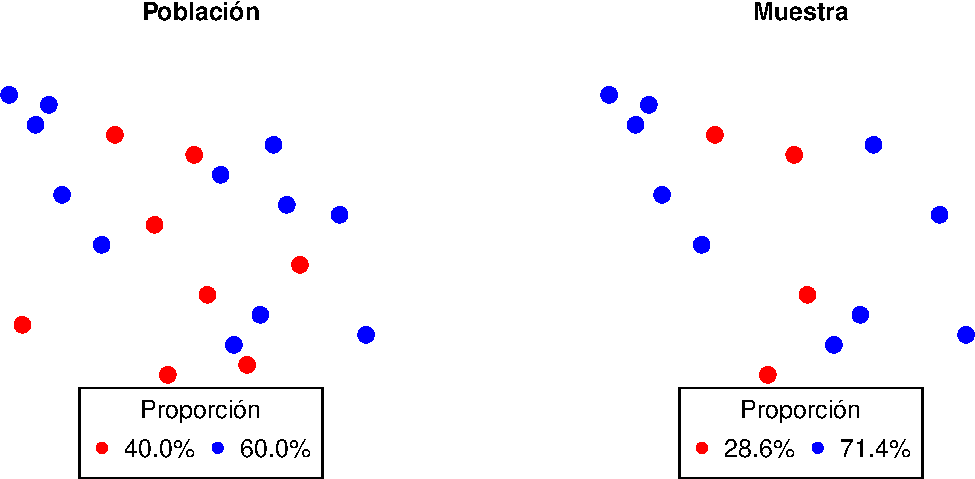
\includegraphics{est1+descriptiva_files/figure-latex/parametro1-1} 

}

\caption{Parámetro y estadístico}\label{fig:parametro1}
\end{figure}

\hypertarget{estimador-y-estimaciuxf3n}{%
\subsection{Estimador y Estimación}\label{estimador-y-estimaciuxf3n}}

Una extensión de los conceptos de parámetro y estadístico, son los de estimador y estimación, para los cuales, se hace la siguiente distinción:

\begin{itemize}
\item
  \textbf{Estimador}: Un estimador es un estadístico usado para aproximar (incertidumbre) el valor de un parámetro. Usualmente no cambia la técnica entre la población y la muestra, por ejemplo, si deseo aproximar la proporción de bolitas rojas en la población, se usaría la proporción de bolitas rojas en la muestra.
\item
  \textbf{Estimación}: Una estimación es el número que resulta de aplicar el estimador a una muestra particular. Esto difiera levemente de la definición anterior, ya que en términos estrictos, el estimador solo es la ``fórmula'', y la estimación es el valor resultante al aplicar la fórmula. Sin embargo, hoy en día es muy común encontrar textos en donde el estimador se considera tanto para la fórmula como para el valor obtenido.
\end{itemize}

Si consideramos un ejemplo similar al anterior (Figura \ref{fig:parametro2}), y establecemos que el \textbf{parámetro} a estudiar es la proporción de círculos rojos, es natural pensar que en la muestra (\textbf{estadístico}) el comportamiento debería ser similar. La intención de decir ``usaremos la proporción de círculos rojos en la muestra para deducir como es la proporción de círculos rojos en la población'' corresponde al \textbf{estimador} (otro tema es argumentar si esto es correcto o no), mientras que, el cálculo del estimador (cálculo de la proporción de círculos rojos en la muestra) lleva el nombre de \textbf{estimación}.

Respecto a lo anterior:

\begin{itemize}
\tightlist
\item
  ¿Cuál sería la estimación de los círculos rojos?
\item
  Si observamos la muestra de la figura \ref{fig:parametro1} y \ref{fig:parametro2}, ¿cuándo diríamos que una estimación es buena?
\end{itemize}

\begin{figure}

{\centering 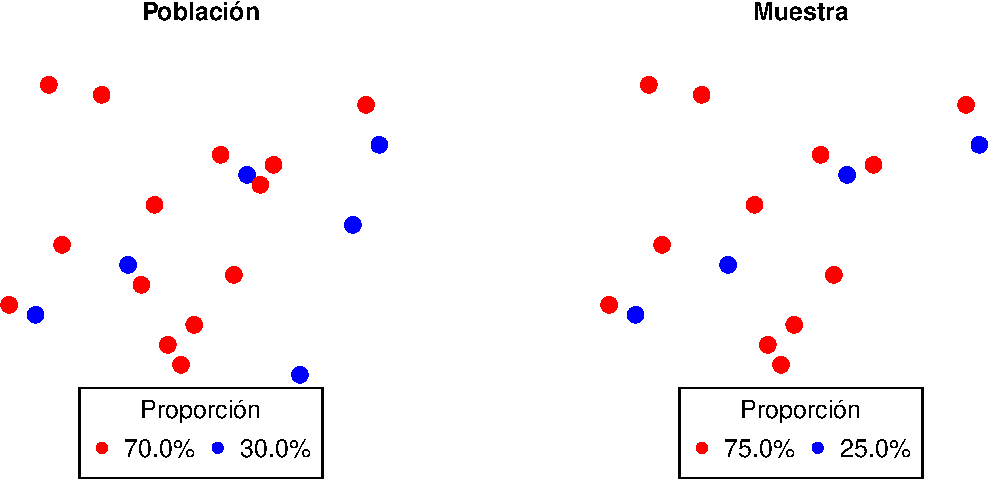
\includegraphics{est1+descriptiva_files/figure-latex/parametro2-1} 

}

\caption{Estimador y estimación}\label{fig:parametro2}
\end{figure}

\hypertarget{variabilidad-muestral}{%
\subsection{Variabilidad muestral}\label{variabilidad-muestral}}

Efectivamente, la estimación de un parámetro está determinada por la muestra con la que se trabaja. La forma en la que se elige una muestra es azarosa (que no se puede intencionar en su totalidad), por lo que es imposible saber de antemano si la estimación será buena o mala respecto al parámetro (error de estimación). En estadística, la forma en la que se elige o genera una muestra puede llegar a ser muy compleja, siendo un tema que está fuera del alcance de este curso.

El concepto detrás de esto es la \textbf{variabilidad muestral}, el cual, indica que dependiendo de la muestra que se obtenga de la población, esta se comportará distinto en relación al estadístico (igualmente para el valor del estimador: estimación). Para ilustrar esto, observemos la figura \ref{fig:figura-poblacion1}.

\textbf{¿Cuál es la proporción de círculos rojos en la población reflejada en la figura} \textbf{?}

\begin{figure}

{\centering 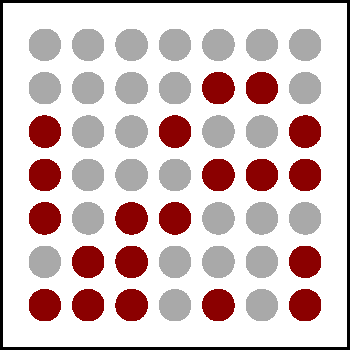
\includegraphics{est1+descriptiva_files/figure-latex/figura-poblacion1-1} 

}

\caption{Población}\label{fig:figura-poblacion1}
\end{figure}

Luego,

\textbf{¿qué podríamos inferir sobre el color predominante en la población en base a la muestra de la figura} \ref{fig:figura-muestra1}\textbf{?}

\begin{figure}

{\centering 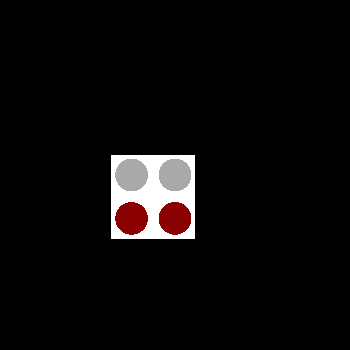
\includegraphics{est1+descriptiva_files/figure-latex/figura-muestra1-1} 

}

\caption{Muestra 1}\label{fig:figura-muestra1}
\end{figure}

\textbf{¿Y ahora? (Figura} \ref{fig:figura-muestra2}\textbf{)}

\begin{figure}

{\centering 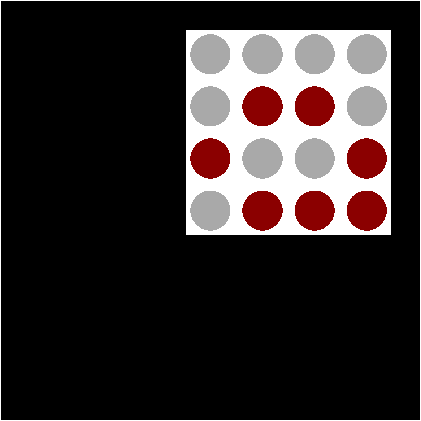
\includegraphics{est1+descriptiva_files/figure-latex/figura-muestra2-1} 

}

\caption{Muestra 2}\label{fig:figura-muestra2}
\end{figure}

Efectivamente, diferentes muestras se comportan de manera diferente, es decir, la estimación depende de la selección de la muestra. Esto se denomina como \textbf{variabilidad muestral}.

\hypertarget{representatividad-y-sesgo-de-la-muestra}{%
\subsection{Representatividad y sesgo de la muestra}\label{representatividad-y-sesgo-de-la-muestra}}

Ambos conceptos se usan con frecuencia en la vida cotidiana, y a su vez están mal empleados. El sesgo no es una propiedad de la muestra sino que del estimador (concepto avanzado de estadística).

Por otro lado, la representatividad no es un concepto válido matemáticamente (no existe tal definición).

\hypertarget{medidas-de-localizaciuxf3n}{%
\subsection{Medidas de localización}\label{medidas-de-localizaciuxf3n}}

Los resúmenes visuales de datos son herramientas excelentes para obtener impresiones y percepciones preliminares. Un análisis de datos más formal a menudo requiere el cálculo e interpretación de medidas de resumen numéricas. Es decir, de los datos se trata de extraer varios números resumidos, números que podrían servir para caracterizar el conjunto de datos. Las tres medidas de resumen más utilizadas son la media, la medianda y la moda.

\hypertarget{media}{%
\subsubsection*{Media}\label{media}}
\addcontentsline{toc}{subsubsection}{Media}

Para un conjunto dado de números \(x_1, x_2, x_3, \ldots, x_n\), la medida más conocida y útil es la \textbf{media} o promedio aritmético. Usualmente se asume que los números \(x_i\) hace parte de una muestra, por lo que a este promedio se le connota como \textbf{media muestral} y se denota con por \(\bar{x}\).

De lo anterior, la media muestral (\(\bar{x}\)) de una conjunto de datos \(x_1, x_2, x_3, \ldots, x_n\) está dada por \citep[página 25]{Devore}

\begin{equation}
\bar{x} = \frac{x_1 + x_2 + \cdots + x_n}{n} = \frac{\displaystyle\sum_{i=1}^{n}x_i}{n}
\label{eq:promedio}
\end{equation}

En R, para obtener el promedio aritmético de los datos se hace uso de la función \textbf{mean()}. A continuación, un ejemplo.

\begin{Shaded}
\begin{Highlighting}[]
\CommentTok{\# Un conjunto de datos cualquiera}
\NormalTok{x }\OtherTok{=} \FunctionTok{c}\NormalTok{(}\DecValTok{1}\NormalTok{,}\DecValTok{2}\NormalTok{,}\DecValTok{3}\NormalTok{,}\DecValTok{6}\NormalTok{,}\DecValTok{1}\NormalTok{,}\SpecialCharTok{{-}}\DecValTok{4}\NormalTok{,}\SpecialCharTok{{-}}\DecValTok{2}\NormalTok{,}\DecValTok{6}\NormalTok{,}\DecValTok{0}\NormalTok{,}\DecValTok{10}\NormalTok{,}\SpecialCharTok{{-}}\DecValTok{20}\NormalTok{)}
\CommentTok{\# Promedio de los datos}
\FunctionTok{mean}\NormalTok{(x)}
\end{Highlighting}
\end{Shaded}

\begin{verbatim}
## [1] 0.2727273
\end{verbatim}

El promedio (\(\bar{x}\)) representa el valor central de las observaciones incluidas en una muestra. Sin embargo, esta medida puede llegar a ser inapropiada en algunas circunstancias, específicamente cuando existen valores extremos. Un ejemplo de esto, es el promedio de los ingresos (\href{https://www.ine.gob.cl/prensa/detalle-prensa/2022/07/21/el-ingreso-laboral-promedio-mensual-en-chile-fue-de-$681.039-en-2021\#:~:text=El\%20ingreso\%20laboral\%20promedio\%20mensual\%20en\%20Chile\%20fue\%20de\%20\%24681.039\%20en\%202021,-21\%2F07\%2F2022\&text=El\%2050\%25\%20de\%20las\%20personas,ingreso\%20de\%20hasta\%20\%24457.690\%20mensuales.}{el caso de Chile}), ya que, es común que unos cuantos afortunados ganen cantidades astronómicas, por lo que el uso del ingreso promedio como medida de resumen puede ser engañoso (otro ejemplo, \href{https://www.google.com/finance/quote/BTC-USD?sa=X\&ved=2ahUKEwi3po-_m9n8AhWUL7kGHTNFCfYQ-fUHegQIFhAe\&window=MAX}{es la valorización de BitCoin al dólar estadounidense}).

A pesar de lo anterior, esta medida sigue siendo ampliamente utilizada, en gran medida porque existen muchas poblaciones para las cuales un valor extremo en la muestra sería altamente improbable (ejemplo: \href{https://www.google.com/finance/quote/EUR-CLP?window=MAX\&comparison=USD-CLP}{tipo de cambio del dólar y el euro}).

\textbf{Ejercicio:}

\begin{enumerate}
\def\labelenumi{\arabic{enumi}.}
\tightlist
\item
  Utilizando la base de datos de la unidad, obtenga la media de la variable (columna) \textbf{Open}. Interprete.
\item
  Utilice el comando \textbf{colMeans()} para obtener la media de todas las variables asociadas a la tasa de conversión (ignore la columna asociada a la variable fecha). Interprete
\end{enumerate}

\hypertarget{mediana}{%
\subsubsection*{Mediana}\label{mediana}}
\addcontentsline{toc}{subsubsection}{Mediana}

La palabra mediana es sinónimo de ``medio'' y la mediana muestral es en realidad el valor medio una vez que se ordenan las observaciones de la más pequeña a la más grande \citep[página 26]{Devore}.

La mediana muestral se obtiene ordenando primero las observaciones de la más pequeña a la más grande. Por lo tanto,

\begin{itemize}
\tightlist
\item
  Si la cantidad de datos es impar, entonces, la mediana es igual al número en la posición \(\frac{n+1}{2}\).
\item
  Si la cantidad de datos es par, entonces, la mediana es el promedio entre los números ubicados en las posiciones \(\frac{n}{2}\) y \((\frac{n}{2}+1)\).
\end{itemize}

Para poder calcular la mediana en R, se debe hacer uso del comando \textbf{median()}, tal como se muestra a continuación.

\begin{Shaded}
\begin{Highlighting}[]
\CommentTok{\# Conjunto de datos (cantidad impar)}
\NormalTok{x }\OtherTok{=} \FunctionTok{c}\NormalTok{(}\DecValTok{1}\NormalTok{,}\DecValTok{2}\NormalTok{,}\DecValTok{3}\NormalTok{,}\DecValTok{4}\NormalTok{,}\DecValTok{5}\NormalTok{,}\DecValTok{6}\NormalTok{,}\DecValTok{7}\NormalTok{,}\SpecialCharTok{{-}}\DecValTok{3}\NormalTok{,}\SpecialCharTok{{-}}\DecValTok{1}\NormalTok{,}\SpecialCharTok{{-}}\DecValTok{2}\NormalTok{,}\FloatTok{5.4}\NormalTok{,}\FloatTok{9.3}\NormalTok{,}\DecValTok{0}\NormalTok{)}
\CommentTok{\# Mediana del conjunto de datos}
\FunctionTok{median}\NormalTok{(x)}
\end{Highlighting}
\end{Shaded}

\begin{verbatim}
## [1] 3
\end{verbatim}

\begin{Shaded}
\begin{Highlighting}[]
\CommentTok{\# Conjunto de datos (cantidad par)}
\NormalTok{x }\OtherTok{=} \FunctionTok{c}\NormalTok{(}\DecValTok{1}\NormalTok{,}\DecValTok{2}\NormalTok{,}\DecValTok{3}\NormalTok{,}\DecValTok{4}\NormalTok{,}\DecValTok{5}\NormalTok{,}\DecValTok{6}\NormalTok{,}\DecValTok{7}\NormalTok{,}\SpecialCharTok{{-}}\DecValTok{3}\NormalTok{,}\SpecialCharTok{{-}}\DecValTok{1}\NormalTok{,}\SpecialCharTok{{-}}\DecValTok{2}\NormalTok{,}\FloatTok{5.4}\NormalTok{,}\FloatTok{9.3}\NormalTok{)}
\CommentTok{\# Mediana del conjunto de datos}
\FunctionTok{median}\NormalTok{(x)}
\end{Highlighting}
\end{Shaded}

\begin{verbatim}
## [1] 3.5
\end{verbatim}

En ambos casos, se entiende que, ordenando los datos de menor a mayor (en una recta real), tanto a la derecha como izquierda de la mediana se encuentra la misma cantidad de datos.

\textbf{Ejercicio:}

\begin{enumerate}
\def\labelenumi{\arabic{enumi}.}
\tightlist
\item
  Utilizando la base de datos de la unidad, determine la mediana de cada una de las variables presentes en la base (ignore la columna asociada a la variable fecha). Interprete.
\end{enumerate}

\hypertarget{moda}{%
\subsubsection*{Moda}\label{moda}}
\addcontentsline{toc}{subsubsection}{Moda}

La moda es la medida más intuitiva de las tres, ya que simplemente corresponde al valor que se presenta con mayor frecuencia \citep[página 85]{anderson}. Para ilustrar esto, veamos el siguiente código en R:

\begin{Shaded}
\begin{Highlighting}[]
\CommentTok{\# El siguiente vector contiene la información de la cantidad de hermanos }
\CommentTok{\# de un determinado grupo de personas}
\NormalTok{hermanos }\OtherTok{=} \FunctionTok{c}\NormalTok{(}\DecValTok{1}\NormalTok{,}\DecValTok{2}\NormalTok{,}\DecValTok{3}\NormalTok{,}\DecValTok{1}\NormalTok{,}\DecValTok{2}\NormalTok{,}\DecValTok{3}\NormalTok{,}\DecValTok{3}\NormalTok{,}\DecValTok{3}\NormalTok{,}\DecValTok{4}\NormalTok{,}\DecValTok{1}\NormalTok{,}\DecValTok{7}\NormalTok{,}\DecValTok{1}\NormalTok{,}\DecValTok{0}\NormalTok{,}\DecValTok{0}\NormalTok{,}\DecValTok{1}\NormalTok{,}\DecValTok{0}\NormalTok{,}\DecValTok{2}\NormalTok{)}
\CommentTok{\# Utilizando el comando table podemos obtener la frecuencia de cada una }
\CommentTok{\# de las distintas observaciones}
\FunctionTok{table}\NormalTok{(hermanos)}
\end{Highlighting}
\end{Shaded}

\begin{verbatim}
## hermanos
## 0 1 2 3 4 7 
## 3 5 3 4 1 1
\end{verbatim}

\begin{Shaded}
\begin{Highlighting}[]
\CommentTok{\# Como resultado se aprecia que la cantidad de hermanos que más se repita dentro }
\CommentTok{\# del grupo de personas es de 5}
\end{Highlighting}
\end{Shaded}

\textbf{Ejemplo:}

\begin{enumerate}
\def\labelenumi{\arabic{enumi}.}
\tightlist
\item
  Cree un objeto que guarde la tabla de frecuencias de la variable Open de la base de datos de la unidad (sin imprimir la tabla).
\end{enumerate}

\begin{Shaded}
\begin{Highlighting}[]
\NormalTok{tabla }\OtherTok{=} \FunctionTok{table}\NormalTok{(datos}\SpecialCharTok{$}\NormalTok{Open)}
\end{Highlighting}
\end{Shaded}

\begin{enumerate}
\def\labelenumi{\arabic{enumi}.}
\setcounter{enumi}{1}
\tightlist
\item
  Ya que es imposible buscar manualmente la frecuencia más alta, utilice el comando \textbf{which.max()} para encontrar la posición en la que se ubica esta, ingresando como argumento la tabla anteriormente guardada. Guarde este valor en un objeto.
\end{enumerate}

\begin{Shaded}
\begin{Highlighting}[]
\NormalTok{(}\AttributeTok{posicion =} \FunctionTok{which.max}\NormalTok{(tabla))}
\end{Highlighting}
\end{Shaded}

\begin{verbatim}
## 1.336005 
##     3067
\end{verbatim}

\begin{enumerate}
\def\labelenumi{\arabic{enumi}.}
\setcounter{enumi}{2}
\tightlist
\item
  Finalmente, consulte de manera directa en la tabla en valor de la frecuencia en la posición calculada en el paso anterior. Interprete.
\end{enumerate}

\begin{Shaded}
\begin{Highlighting}[]
\NormalTok{tabla[posicion]}
\end{Highlighting}
\end{Shaded}

\begin{verbatim}
## 1.336005 
##        6
\end{verbatim}

Esto quiere decir, que el valor de apertura de la tasa EUR/USD que más se repite históricamente es 1.336005 con una frecuencia de 6.

\emph{Nota: En caso de que existan dos o más valores con las frecuencias más altas, el programa solo reporta la primera, según el orden lexicográfico de las columnas.}

\textbf{Ejercicio:}

\begin{enumerate}
\def\labelenumi{\arabic{enumi}.}
\tightlist
\item
  Replique los anterior para el resto de variables presentes en la base de datos de la unidad (ignore la columna asociada a la variable fecha).
\end{enumerate}

\textbf{Nota}: en el documento se usará simplemente el nombre de la medida de localización (media, moda, mediana) para referirse a la medida de localización muestral. En casos determinados se hará la distinción entre el caso muestral y poblacional, según corresponda (ejemplo: media poblacional, media muestral).

\hypertarget{medidas-de-escala}{%
\subsection{Medidas de escala}\label{medidas-de-escala}}

Al momento de reportar la media solo se obtiene información parcial sobre el un conjunto de datos. Diferentes muestras o poblaciones pueden tener medidas idénticas de localización y aún diferir entre sí en otras importantes maneras. La tabla \ref{tab:variabilidad} muestra las notas obtenidas por los alumnos de 2 dos cursos con la misma media, aunque el grado de \textbf{dispersión} (variabilidad) en torno a esta es diferente para ambas muestras, es decir, en el Curso 1 las se observan notas más bajas y altas que el Curso 2.

\begin{table}

\caption{\label{tab:variabilidad}Notas por curso}
\centering
\begin{tabular}[t]{ccc}
\toprule
Curso 1 & Curso 2 & Curso 3\\
\midrule
3.0 & 4.0 & 3.0\\
4.5 & 5.0 & 7.0\\
5.0 & 6.0 & --\\
5.5 & -- & --\\
7.0 & -- & --\\
\bottomrule
\end{tabular}
\end{table}

\hypertarget{rango}{%
\subsubsection*{Rango}\label{rango}}
\addcontentsline{toc}{subsubsection}{Rango}

La medida más simple de variabilidad en una muestra es el \textbf{rango}, el cual es la diferencia entre los valores muestrales más grande y más pequeño \citep[página 32]{Devore}. El rango de las notas del curso 1 en la tabla \ref{tab:variabilidad} es más grande que el del curso 2, lo que refleja más variabilidad en la primer muestra que en la segunda. Un defecto del rango, no obstante, es que depende de solo las dos observaciones más extremas y hace caso omiso de las posiciones de los valores restantes. Los cursos 1 y 3 tienen rangos idénticos, aunque cuando se toman en cuenta las observaciones entre los dos extremos, existe mucho menos variabilidad o dispersión en la tercera muestra que en la primera.

\textbf{Ejemplo:}

Obtengamos el rango de la tasa de apertura histórica del EUR/USD de la base de datos de la undiad.

\begin{Shaded}
\begin{Highlighting}[]
\CommentTok{\# Utilizando el comando range() se obtienen los valores mínimo y máximo}
\CommentTok{\# de la variable en cuestión}
\NormalTok{(}\AttributeTok{rango =} \FunctionTok{range}\NormalTok{(datos}\SpecialCharTok{$}\NormalTok{Open))}
\end{Highlighting}
\end{Shaded}

\begin{verbatim}
## [1] 0.959619 1.598184
\end{verbatim}

\begin{Shaded}
\begin{Highlighting}[]
\CommentTok{\# Luego calculamos la diferencia entre el valor máximo y mínimo}
\NormalTok{rango[}\DecValTok{2}\NormalTok{] }\SpecialCharTok{{-}}\NormalTok{ rango[}\DecValTok{1}\NormalTok{]}
\end{Highlighting}
\end{Shaded}

\begin{verbatim}
## [1] 0.638565
\end{verbatim}

\begin{Shaded}
\begin{Highlighting}[]
\CommentTok{\# Nota: El valor máximo siempre estará en la segunda posición y le mínimo en la segunda.}
\end{Highlighting}
\end{Shaded}

\textbf{Ejercicio:}

\begin{enumerate}
\def\labelenumi{\arabic{enumi}.}
\tightlist
\item
  Obtener el rango del resto de variables de la base de datos de la undiad (ignore la columna asociada a la variable fecha).
\end{enumerate}

\hypertarget{varianza-y-desviaciuxf3n-estuxe1ndar}{%
\subsubsection*{Varianza y desviación estándar}\label{varianza-y-desviaciuxf3n-estuxe1ndar}}
\addcontentsline{toc}{subsubsection}{Varianza y desviación estándar}

Las medidas principales de variabilidad implican las \textbf{desviaciones de la media},

\begin{equation}
x_1 - \bar{x}, x_2 - \bar{x}, x_3 - \bar{x}, \ldots, x_n - \bar{x}.
\label{eq:desviaciones}
\end{equation}

Es decir, las desviaciones de la media se obtienen restando \(\bar{x}\) de cada una de las \(n\) observaciones muestrales. Una desviación será positiva si la observación es más grande que la media (a la derecha de la media sobre la recta real) y negativa si la observación es más pequeña que la media (a la izquierda de la media sobre la recta real). Si todas las desviaciones son pequeñas en magnitud, entonces todos los valores de la muestra son cercanos a la media y hay poca variabilidad. Alternativamente, si algunas de las desviaciones son grandes de magnitud, entonces algunos de los de los valores de la muestra están lejos de la media (sobre la recta real) lo que sugiere una mayor variabilidad.

Una forma de resumir las desviaciones sería sumando todas ellas. Sin embargo, es una mala idea, ya que la suma siempre es igual a cero \eqref{eq:sumadesviaciones}, ¿alguna idea del por qué?

\begin{equation}
\text{Suma de las desviaciones en una muestra} = \sum_{i=1}^{n}(x_i-\bar{x}) = 0
\label{eq:sumadesviaciones}
\end{equation}

En este sentido, para poder resumir las desviaciones de una muestra evitando el problema mencionado, se elaboran dos expresiones \citep[página 32]{Devore}:

\begin{itemize}
\tightlist
\item
  Varianza (muestral):
\end{itemize}

\begin{equation}
S^2= \frac{1}{n-1}\sum_{i=1}^{n}(x_i-\bar{x})^2
\label{eq:varianzamuestral}
\end{equation}

\begin{itemize}
\tightlist
\item
  Desviación estándar (muestral):
\end{itemize}

\begin{equation}
S = \sqrt{S^2}
\label{eq:demuestral}
\end{equation}

Las unidades correspondientes a la \textbf{varianza} suele causar confusión. Como los valores que se suman para calcular la varianza, \((x_i-\bar{x})^2\), están elevados al cuadrado, las unidades correspondientes a la varianza muestral también están elevadas al cuadrado. Las unidades al cuadrado de la varianza dificulta la compresión e interpretación intuitiva de los valores numéricos de la varianzas. Lo recomendable es entender la varianza como una medida útil para comparar la variabilidad de dos o más variables. Al comparar variables, la que tiene la varianza mayor, muestra más variabilidad. Otra interpretación del valor de la varianza suele ser innecesaria \citep[página 94]{anderson}.

La \textbf{desviación estándar} es la raíz cuadrada de la varianza, pero, ¿qué se gana con esto? Al calcular la desviación estándar, las unidades de esta son iguales a de la variable original, por lo que es más fácil de interpretar. Sin embargo, estas dos medidas tiene ciertas limitantes a la hora de comprar la variabilidad de dos variables:

\begin{enumerate}
\def\labelenumi{\arabic{enumi}.}
\tightlist
\item
  Es ideal que ambas variable tengan la misma media.
\item
  Las variables deben tener la misma unidad de medida.
\end{enumerate}

No seguir estas recomendaciones puede generar un falsa sensación en la comunicación de resultados.

\textbf{Ejemplo:}

Compare la variabilidad entre la tasa de apertura y la tasa de cierre histórica del EUR/USD presentes en la base de datos de la unidad, para ello:

\begin{enumerate}
\def\labelenumi{\arabic{enumi}.}
\tightlist
\item
  Verifique la media de ambas variables la misma
\end{enumerate}

\begin{Shaded}
\begin{Highlighting}[]
\FunctionTok{mean}\NormalTok{(datos}\SpecialCharTok{$}\NormalTok{Open) }\CommentTok{\# Promedio de la tasa de apertura}
\end{Highlighting}
\end{Shaded}

\begin{verbatim}
## [1] 1.244338
\end{verbatim}

\begin{Shaded}
\begin{Highlighting}[]
\FunctionTok{mean}\NormalTok{(datos}\SpecialCharTok{$}\NormalTok{Close) }\CommentTok{\# Promedio de la tasa de cierre}
\end{Highlighting}
\end{Shaded}

\begin{verbatim}
## [1] 1.244363
\end{verbatim}

\begin{Shaded}
\begin{Highlighting}[]
\CommentTok{\# Las tasas son similares hasta el tercer decimal, se asumirá que las medias son iguales}
\end{Highlighting}
\end{Shaded}

\begin{enumerate}
\def\labelenumi{\arabic{enumi}.}
\setcounter{enumi}{1}
\tightlist
\item
  Ya que tienen la misma unidad de medida, calcule la varianza y desviación estándar de cada una. Interprete.
\end{enumerate}

\begin{Shaded}
\begin{Highlighting}[]
\CommentTok{\# Al calcular la varianza muestral, se observa que la tasa de cierre es levemente menor}
\CommentTok{\# variabilidad que la tasa de apertura.}
\FunctionTok{c}\NormalTok{(}\FunctionTok{var}\NormalTok{(datos}\SpecialCharTok{$}\NormalTok{Open), }\FunctionTok{var}\NormalTok{(datos}\SpecialCharTok{$}\NormalTok{Close))}
\end{Highlighting}
\end{Shaded}

\begin{verbatim}
## [1] 0.01562596 0.01562404
\end{verbatim}

\begin{Shaded}
\begin{Highlighting}[]
\CommentTok{\# Al calcular la desviación estándar muestral, se observa que la tasa de cierre tiene menor}
\CommentTok{\# variabilidad que la tasa de apertura.}
\FunctionTok{c}\NormalTok{(}\FunctionTok{sd}\NormalTok{(datos}\SpecialCharTok{$}\NormalTok{Open), }\FunctionTok{sd}\NormalTok{(datos}\SpecialCharTok{$}\NormalTok{Close))}
\end{Highlighting}
\end{Shaded}

\begin{verbatim}
## [1] 0.1250038 0.1249962
\end{verbatim}

\begin{Shaded}
\begin{Highlighting}[]
\CommentTok{\# ¿Por qué es más clara la interpretación (primer decimal distinto) al utilizar}
\CommentTok{\# la desviación estándar?}
\end{Highlighting}
\end{Shaded}

\textbf{Ejercicio:}

\begin{enumerate}
\def\labelenumi{\arabic{enumi}.}
\tightlist
\item
  Utilice la varianza directamente para comparar la variabilidad entre la tasa de apertura y la tasa más alta histórica del EUR/USD presentes en la base de datos de la unidad.
\end{enumerate}

\hypertarget{coeficiente-de-variaciuxf3n}{%
\subsubsection*{Coeficiente de variación}\label{coeficiente-de-variaciuxf3n}}
\addcontentsline{toc}{subsubsection}{Coeficiente de variación}

Para subsanar el problema de las limitaciones de la varianza y desviación estándar, se encuentra la medida llamada \textbf{coeficiente de variación} \eqref{eq:cv}.

\begin{equation}
CV = \left(\frac{S}{|\bar{x}|}\right)\cdot 100\%
\label{eq:cv}
\end{equation}

Cuando el valor del coeficiente de variación es cercano a 100\% se habla de mayor dispersión (heterogéneo), mientras que un valor cercano a 0\% indica menor dispersión (homogéneo), además, se debe considerar que el porcentaje calculado corresponde a la variabilidad respecto a la media de los datos. Sin embargo, no es recomendable usar esta medida cuando el valor de la media es cercano a cero, ya que el CV pierde su significado al tomar valores muy grandes, lo que daría una falsa sensación de dispersión de los datos \citep[página 95]{anderson}.

\textbf{Ejemplo:}

En el ejercicio anterior, se utilizó la varianza para comprar directamente la variabilidad entre la tasa de apertura y la tasa más alta histórica del EUR/USD. Sin embargo, si calculamos las medias de ambas variables se puede verificar que son distintas. Utilice el CV para comprar la variabilidad de ambas variables.

\begin{Shaded}
\begin{Highlighting}[]
\CommentTok{\# Claramente la media de la tasa más alta es mayor a la media de la tasa de apertura.}
\FunctionTok{c}\NormalTok{(}\FunctionTok{mean}\NormalTok{(datos}\SpecialCharTok{$}\NormalTok{Open), }\FunctionTok{mean}\NormalTok{(datos}\SpecialCharTok{$}\NormalTok{High))}
\end{Highlighting}
\end{Shaded}

\begin{verbatim}
## [1] 1.244338 1.249022
\end{verbatim}

\begin{Shaded}
\begin{Highlighting}[]
\CommentTok{\# Al verificarse una de las dos limitantes mencionadas, procedemos}
\CommentTok{\# a calcular el CV de ambas variables}
\NormalTok{CV\_Open }\OtherTok{=} \FunctionTok{sd}\NormalTok{(datos}\SpecialCharTok{$}\NormalTok{Open)}\SpecialCharTok{/}\FunctionTok{abs}\NormalTok{(}\FunctionTok{mean}\NormalTok{(datos}\SpecialCharTok{$}\NormalTok{Open))}\SpecialCharTok{*}\DecValTok{100}
\NormalTok{CV\_High }\OtherTok{=} \FunctionTok{sd}\NormalTok{(datos}\SpecialCharTok{$}\NormalTok{High)}\SpecialCharTok{/}\FunctionTok{abs}\NormalTok{(}\FunctionTok{mean}\NormalTok{(datos}\SpecialCharTok{$}\NormalTok{High))}\SpecialCharTok{*}\DecValTok{100}
\FunctionTok{c}\NormalTok{(CV\_Open, CV\_High)}
\end{Highlighting}
\end{Shaded}

\begin{verbatim}
## [1] 10.04581 10.06323
\end{verbatim}

\begin{Shaded}
\begin{Highlighting}[]
\CommentTok{\# Se puede observar que el coeficiente de variabilidad de la tasa más alta (10.06\%)}
\CommentTok{\# es mayor a la de la tasa de apertura (10.04\%). Por lo tanto, }
\CommentTok{\# la variabilidad (dispersión) de los datos es más homogénea para la tasa de}
\CommentTok{\# apertura. Sin embargo, la diferencia es muy pequeña, por lo que la dispersión en }
\CommentTok{\# relación a la media es similar entre ambas variables.}
\end{Highlighting}
\end{Shaded}

\textbf{Ejercicio:}

\begin{enumerate}
\def\labelenumi{\arabic{enumi}.}
\tightlist
\item
  Comparar la variabilidad entre la tasa de más baja y de cierre histórica del EUR/USD presentes en la base de datos de la unidad. Interprete.
\end{enumerate}

\textbf{Nota}: en el documento se usará simplemente el nombre de la medida de escala (rango, varianza, desviación estándar y CV) para referirse a la medida de escala muestral. En casos determinados se hará la distinción entre el caso muestral y poblacional, según corresponda (ejemplo: varianza poblacional, varianza muestral).

\hypertarget{notaciuxf3n-poblacional-y-muestral}{%
\subsubsection*{Notación poblacional y muestral}\label{notaciuxf3n-poblacional-y-muestral}}
\addcontentsline{toc}{subsubsection}{Notación poblacional y muestral}

\begin{table}

\caption{\label{tab:notacion}Notación de parámetros y estadísticos}
\centering
\begin{tabular}[t]{lcc}
\toprule
  & Poblacional & Muestral\\
\midrule
Media & $\mu$ & $\bar{x}$\\
Varianza & $\sigma^2$ & $S^2$\\
Desviación estándar & $\sigma$ & $S$\\
\bottomrule
\end{tabular}
\end{table}

\hypertarget{gruxe1ficos-descriptivos}{%
\section{Gráficos descriptivos}\label{gruxe1ficos-descriptivos}}

En este apartado, se considera la representación de un conjunto de datos por medio de técnicas visuales. A continuación, se hará mención de algunas de las técnicas más útiles y pertinentes a la estadística de descriptiva. Los ejemplos presentados en esta sección hacen uso de la base de datos de la unidad (sección \ref{unidad1}).

\hypertarget{histograma}{%
\subsection{Histograma}\label{histograma}}

Algunos datos numéricos se obtienen contando para determinar el valor de una variable (cuántas veces se repite un hecho), mientras que otro datos se obtienen tomando mediciones (peso, altura, tiempo de reacción). Usualmente, este tipo de gráfico se utiliza con datos continuos (aunque tiene una versión para datos discretos), para lo cual, se debe hacer lo siguiente \citep[página 12]{Devore}:

\begin{enumerate}
\def\labelenumi{\arabic{enumi}.}
\tightlist
\item
  Subdividir los datos en \textbf{intervalos de clase} o \textbf{clases}, de tal manera que cada observación quede contenida en exactamente una clase. Para esto, se hace uso de la regla de Sturges \citeyearpar{sturges1926choice}, la cual, consiste en calcular la expresión \(1+\log_2(n)\), aproximando hacia el entero más próximo, dónde \(n\) corresponde a la cantidad de datos (existen otra variedad de técnicas).
\item
  Determinar la frecuencia y la frecuencia relativa de cada clase, es decir, cuántas observaciones hay en cada uno de los intervalos.
\item
  Se marcan los límite de clase sobre el eje horizontal del plano cartesiano.
\item
  Se traza un rectángulo cuya altura es la frecuencia absoluta (o relativa) correspondiente a cada intervalo de clase.
\end{enumerate}

Para generar un histograma en R a partir de un conjunto de datos, se utiliza el siguiente código:

\begin{Shaded}
\begin{Highlighting}[]
\FunctionTok{library}\NormalTok{(ggplot2) }\CommentTok{\# Librería de ggplot2}
\FunctionTok{ggplot}\NormalTok{( }\CommentTok{\# Ambiente gráfico}
  \AttributeTok{data =}\NormalTok{ datos, }\CommentTok{\# Base de datos a utilizar}
       \FunctionTok{aes}\NormalTok{( }\CommentTok{\# Comandos estéticos}
         \AttributeTok{x =}\NormalTok{ Close)) }\SpecialCharTok{+} \CommentTok{\# Eje X y variable asociada }
  \FunctionTok{geom\_histogram}\NormalTok{( }\CommentTok{\# Objeto a graficar: histograma}
    \AttributeTok{bins =} \DecValTok{13}\NormalTok{, }\CommentTok{\# Cantidad de intervalos del histograma}
    \AttributeTok{color =} \StringTok{"white"}\NormalTok{, }\CommentTok{\# Color del borde de las barras del histograma}
    \AttributeTok{fill =} \StringTok{"darkred"}\NormalTok{, }\CommentTok{\# Color de relleno de las barras}
    \AttributeTok{closed =} \StringTok{"left"}\NormalTok{) }\SpecialCharTok{+} \CommentTok{\# Tipo de intervalo del histograma}
  \FunctionTok{labs}\NormalTok{( }\CommentTok{\# Títulos}
    \AttributeTok{title =} \StringTok{"Histograma EUR/USD"}\NormalTok{, }\CommentTok{\# Título del gráfico}
    \AttributeTok{x =} \StringTok{"Tasa de cierre"}\NormalTok{, }\CommentTok{\# Título del eje X}
    \AttributeTok{y =} \StringTok{"Frecuencia"}\NormalTok{) }\CommentTok{\# Título del eje Y}
\end{Highlighting}
\end{Shaded}

\begin{center}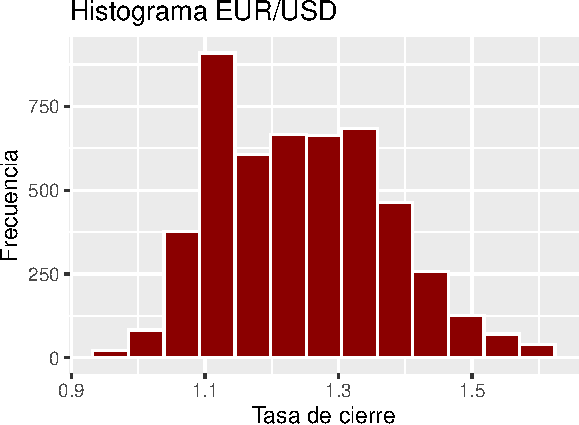
\includegraphics{est1+descriptiva_files/figure-latex/unnamed-chunk-13-1} \end{center}

Es útil recordar que el histograma está asociado a una tabla de frecuencia por intervalos. Para obtener la tabla asociada a un histograma se puede utilizar el siguiente código.

\begin{Shaded}
\begin{Highlighting}[]
\CommentTok{\# Datos del histograma guardados}
\NormalTok{h }\OtherTok{=} \FunctionTok{hist}\NormalTok{(datos}\SpecialCharTok{$}\NormalTok{Close, }\CommentTok{\# Datos a graficar en el histograma}
         \AttributeTok{breaks =} \DecValTok{13}\NormalTok{, }\CommentTok{\# Cantidad de intervalos (Sturges)}
         \AttributeTok{right =}\NormalTok{ F, }\CommentTok{\# Cerrado por la izquierda}
         \AttributeTok{plot =}\NormalTok{ F) }\CommentTok{\# No desplegar el gráfico en consola}
\FunctionTok{library}\NormalTok{(agricolae) }\CommentTok{\# Librería para generar la tabla de frecuencias}
\FunctionTok{print}\NormalTok{(}\FunctionTok{table.freq}\NormalTok{(h)) }\CommentTok{\# Imprime en consola la tabla de frecuencias}
\end{Highlighting}
\end{Shaded}

\begin{verbatim}
##    Lower Upper  Main Frequency Percentage   CF   CPF
## 1   0.95  1.00 0.975        46        0.9   46   0.9
## 2   1.00  1.05 1.025        89        1.8  135   2.7
## 3   1.05  1.10 1.075       444        8.9  579  11.7
## 4   1.10  1.15 1.125       839       16.9 1418  28.6
## 5   1.15  1.20 1.175       591       11.9 2009  40.5
## 6   1.20  1.25 1.225       634       12.8 2643  53.2
## 7   1.25  1.30 1.275       614       12.4 3257  65.6
## 8   1.30  1.35 1.325       654       13.2 3911  78.8
## 9   1.35  1.40 1.375       510       10.3 4421  89.0
## 10  1.40  1.45 1.425       257        5.2 4678  94.2
## 11  1.45  1.50 1.475       166        3.3 4844  97.5
## 12  1.50  1.55 1.525        38        0.8 4882  98.3
## 13  1.55  1.60 1.575        84        1.7 4966 100.0
\end{verbatim}

\textbf{Ejercicio:}

\begin{enumerate}
\def\labelenumi{\arabic{enumi}.}
\tightlist
\item
  Utilizando la variable \textbf{Low} de la base de datos de la unidad, elabore un histograma y obtenga la tabla de frecuencias asociada. Interprete.
\end{enumerate}

\hypertarget{caja}{%
\subsection{Caja}\label{caja}}

El gráfico de caja se utiliza para describir las siguiente características de un conjunto de datos \citep[página 35]{Devore}:

\begin{itemize}
\tightlist
\item
  El centro.
\item
  La dispersión.
\item
  El grado y naturaleza de cualquier alejamiento de la simetría.
\item
  La identificación de las observaciones ``extremas'' (atípicas) inusualmente alejadas del cuerpo principal de los datos.
\end{itemize}

Los pasos para elaborar un gráfico de caja son los siguiente \citep[página 106]{anderson}:

\begin{enumerate}
\def\labelenumi{\arabic{enumi}.}
\tightlist
\item
  Se dibuja una caja cuyos extremos se localicen en primer y tercer cuartiles. Esta caja contiene 50\% de los datos centrales.
\item
  En el punto donde se localiza la mediana se traza una linea horizontal.
\item
  Usando el rango intercuartílico (\(RIC = Q_3-Q_1\)), se localizan los límites. En un gráfico de caja los límites se encuentra a \(1.5RIC\) abajo y arriba de \(Q_1\) y \(Q_3\) respectivamente. Los datos que quedan fuera de estos límites se consideran observaciones atípicas \citep{Tukey}. La razón por la cual se considera 1.5 veces el rango intercuartílico es convencional, no obstante, hay argumento relacionados a la cantidad de datos dentro de los limites inferior y superior, los cuales indican que debe ser de 99.7\% \citep{James2013}.
\item
  Las lineas que se extienden verticalmente desde la caja se les llama \emph{bigotes}. Los bigotes van desde los extremos de la caja hasta los valores menor y mayor de los límites calculados en el paso 3.
\item
  Mediante puntos se indica la localización de las observaciones atípicas.
\end{enumerate}

Para generar un gráfico de caja en R a partir de un conjunto de datos, se utiliza el siguiente código:

\begin{Shaded}
\begin{Highlighting}[]
\NormalTok{g }\OtherTok{=} \FunctionTok{ggplot}\NormalTok{( }\CommentTok{\# Ambiente gráfico}
  \AttributeTok{data =}\NormalTok{ datos, }\CommentTok{\# Base de datos a utilizar}
  \FunctionTok{aes}\NormalTok{( }\CommentTok{\# Comandos estéticos}
    \AttributeTok{y =}\NormalTok{ Close)) }\SpecialCharTok{+} \CommentTok{\# Eje Y y variable asociada}
  \FunctionTok{geom\_boxplot}\NormalTok{( }\CommentTok{\# Objeto a graficar: gráfico de caja}
    \AttributeTok{color =} \StringTok{"black"}\NormalTok{, }\CommentTok{\# Color del borde del gráfico}
    \AttributeTok{fill =} \StringTok{"darkred"}\NormalTok{) }\SpecialCharTok{+} \CommentTok{\# Color de relleno del gráfico}
  \FunctionTok{labs}\NormalTok{( }\CommentTok{\# Títulos }
    \AttributeTok{title =} \StringTok{"Caja EUR/USD (opción 1)"}\NormalTok{, }\CommentTok{\# Título del gráfico}
    \AttributeTok{x =} \StringTok{""}\NormalTok{, }\CommentTok{\# Título del eje X}
    \AttributeTok{y =} \StringTok{"Tasa de cierre"}\NormalTok{) }\SpecialCharTok{+} \CommentTok{\# Título del eje Y}
  \FunctionTok{theme}\NormalTok{( }\CommentTok{\# Aspectos visuales del gráfico}
    \AttributeTok{axis.ticks.x =} \FunctionTok{element\_blank}\NormalTok{(), }\CommentTok{\# Elimina las regletas del eje X}
    \AttributeTok{axis.text.x =} \FunctionTok{element\_blank}\NormalTok{()) }\CommentTok{\# Elimina los números del eje X}
\NormalTok{info }\OtherTok{=} \FunctionTok{unlist}\NormalTok{(}\FunctionTok{ggplot\_build}\NormalTok{(g)[[}\DecValTok{1}\NormalTok{]]) }\CommentTok{\# Guardamos los valores del gráfico}
\NormalTok{values }\OtherTok{=} \FunctionTok{round}\NormalTok{(}\FunctionTok{as.numeric}\NormalTok{(info[}\DecValTok{1}\SpecialCharTok{:}\DecValTok{5}\NormalTok{]), }\DecValTok{3}\NormalTok{) }\CommentTok{\# Extraemos los valores de construcción}
\NormalTok{g1 }\OtherTok{=}\NormalTok{ g }\SpecialCharTok{+} \CommentTok{\# Creamos un nuevo gráfico a partir del anterior}
  \FunctionTok{scale\_y\_continuous}\NormalTok{( }\CommentTok{\# Modificar el eje Y}
    \AttributeTok{breaks =}\NormalTok{ values, }\CommentTok{\# Modificamos los puntos a considerar en el eje Y}
    \AttributeTok{labels =}\NormalTok{ values) }\SpecialCharTok{+} \CommentTok{\# Modificamos los valores mostrados en el eje Y}
  \FunctionTok{labs}\NormalTok{( }\CommentTok{\# Títulos}
    \AttributeTok{title =} \StringTok{"Caja EUR/USD (opción 2)"}\NormalTok{) }\CommentTok{\# Título del gráfico}
\FunctionTok{library}\NormalTok{(gridExtra) }\CommentTok{\# Librería para juntar gráficos de ggplot2}
\FunctionTok{grid.arrange}\NormalTok{(g, }\CommentTok{\# Gráfico}
\NormalTok{             g1, }\CommentTok{\# Gráfico}
             \AttributeTok{ncol =} \DecValTok{2}\NormalTok{) }\CommentTok{\# Despliegue en a dos columnas }
\end{Highlighting}
\end{Shaded}

\begin{center}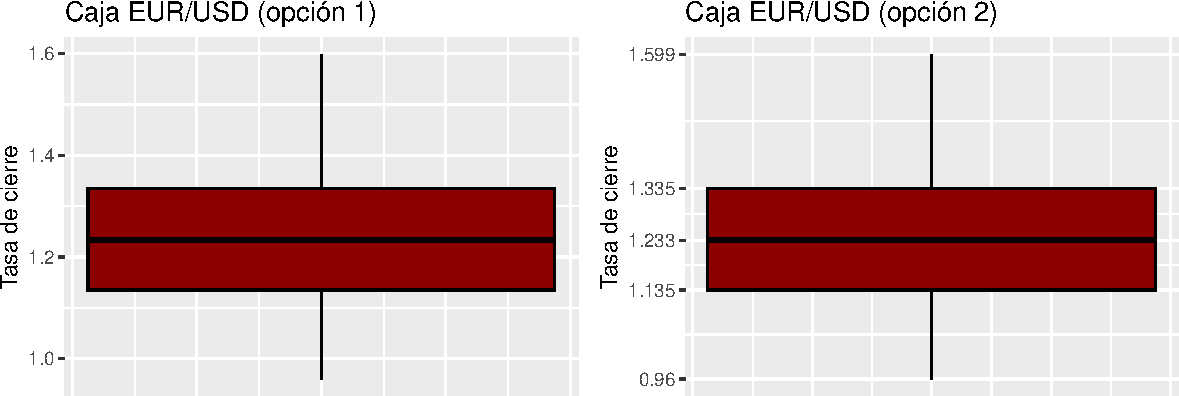
\includegraphics{est1+descriptiva_files/figure-latex/unnamed-chunk-15-1} \end{center}

\textbf{Ejercicio:}

\begin{enumerate}
\def\labelenumi{\arabic{enumi}.}
\tightlist
\item
  Utilizando la variable \textbf{Open} de la base de datos de la unidad, elabore un gráfico de caja. Interprete.
\end{enumerate}

\hypertarget{violuxedn}{%
\subsection{Violín}\label{violuxedn}}

El gráfico de violín proporciona una representación más completa y precisa de la distribución de los datos que las técnicas anteriores, ya que muestra tanto la forma de la distribución como su concentración \citep{hintze1998violin}. La utilidad de este gráfico recae en la comparación de la distribución de los datos entre distintos grupos y/o categorías.

El proceso de construcción del gráfico es el siguiente:

\begin{enumerate}
\def\labelenumi{\arabic{enumi}.}
\tightlist
\item
  Dibujo de la traza de densidad: la traza de densidad se dibuja sobre el eje vertical en el gráfico de violín (``forma suavizada del histograma'').
\item
  Creación de la sección central simétrica: se crea una sección central simétrica que representa la mitad de la traza de densidad.
\end{enumerate}

Adicionalmente, es común agregar un gráfico de caja junto al de violín con el fin de incorporar la visualización de las medidas de posición.

Para generar un gráfico de violín en R a partir de un conjunto de datos, se utiliza el siguiente código:

\begin{Shaded}
\begin{Highlighting}[]
\CommentTok{\# Se guarda el gráfico en una variable para posteriormente}
\CommentTok{\# integrar otros gráficos dentro de este.}
\NormalTok{g }\OtherTok{=} \FunctionTok{ggplot}\NormalTok{( }\CommentTok{\# Ambiente gráfico}
  \AttributeTok{data =}\NormalTok{ datos, }\CommentTok{\# Base de datos a utilizar}
  \FunctionTok{aes}\NormalTok{( }\CommentTok{\# Comandos estéticos}
    \AttributeTok{x =} \DecValTok{1}\NormalTok{, }\CommentTok{\# Se fija el valor horizontal del gráfico (a elección)}
    \AttributeTok{y =}\NormalTok{ Close)) }\SpecialCharTok{+} \CommentTok{\# Eje Y y variable asociada}
  \FunctionTok{geom\_violin}\NormalTok{( }\CommentTok{\# Objeto a graficar: violín}
    \AttributeTok{trim =}\NormalTok{ F, }\CommentTok{\# Modifica las terminaciones visuales superior e inferior}
    \AttributeTok{fill =} \StringTok{"aquamarine3"}\NormalTok{) }\SpecialCharTok{+} \CommentTok{\# Color de relleno del gráfico}
  \FunctionTok{labs}\NormalTok{( }\CommentTok{\# Títulos}
    \AttributeTok{title =} \StringTok{"Violín EUR/USD"}\NormalTok{, }\CommentTok{\# Título del gráfico}
    \AttributeTok{x =} \StringTok{""}\NormalTok{, }\CommentTok{\# Título del eje X}
    \AttributeTok{y =} \StringTok{"Tasa de cierre"}\NormalTok{) }\SpecialCharTok{+} \CommentTok{\# Título del eje Y}
  \FunctionTok{theme}\NormalTok{( }\CommentTok{\# Aspectos visuales del gráfico}
    \AttributeTok{axis.ticks.x =} \FunctionTok{element\_blank}\NormalTok{(), }\CommentTok{\# Elimina las regletas del eje X}
    \AttributeTok{axis.text.x =} \FunctionTok{element\_blank}\NormalTok{()) }\CommentTok{\# Elimina los números del eje X}
\NormalTok{g }\CommentTok{\# Desplegamos el gráfico en el visualizador}
\end{Highlighting}
\end{Shaded}

\begin{center}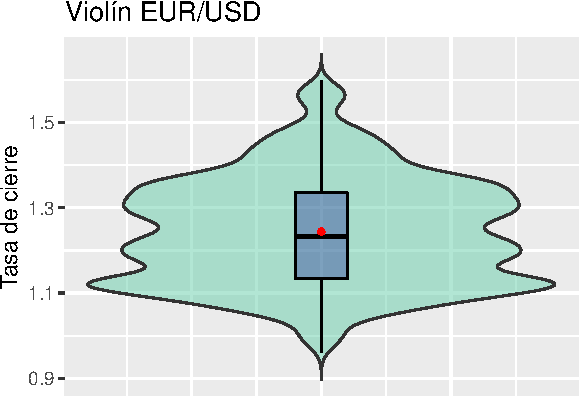
\includegraphics{est1+descriptiva_files/figure-latex/unnamed-chunk-16-1} \end{center}

\begin{Shaded}
\begin{Highlighting}[]
\CommentTok{\# Agregamos otros elementos al gráfico guardado}
\NormalTok{g }\SpecialCharTok{+} \FunctionTok{geom\_boxplot}\NormalTok{( }\CommentTok{\# Objeto a graficar: gráfico de caja}
  \AttributeTok{width =} \FloatTok{0.1}\NormalTok{, }\CommentTok{\# Anchura proporcional del nuevo gráfico de caja}
  \AttributeTok{color =} \StringTok{"black"}\NormalTok{, }\CommentTok{\# Color de borde del gráfico}
  \AttributeTok{fill =} \StringTok{"lightblue2"}\NormalTok{) }\SpecialCharTok{+} \CommentTok{\# Color de relleno del gráfico}
  \FunctionTok{stat\_summary}\NormalTok{( }\CommentTok{\# Función para agregar información de resumen}
    \AttributeTok{fun =}\NormalTok{ mean, }\CommentTok{\# Tipo de información: promedio}
    \AttributeTok{geom =} \StringTok{"point"}\NormalTok{, }\CommentTok{\# Forma visual}
    \AttributeTok{size =} \DecValTok{1}\NormalTok{, }\CommentTok{\# Tamaño}
    \AttributeTok{color =} \StringTok{"red"}\NormalTok{) }\CommentTok{\# Color}
\end{Highlighting}
\end{Shaded}

\begin{center}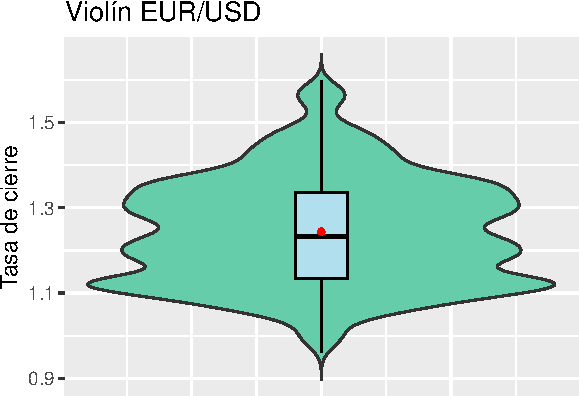
\includegraphics{est1+descriptiva_files/figure-latex/unnamed-chunk-17-1} \end{center}

\textbf{Ejercicio:}

\begin{enumerate}
\def\labelenumi{\arabic{enumi}.}
\tightlist
\item
  Utilizando las variables \textbf{Low} y \textbf{Open} de la base de datos de la unidad, elabore un gráfico violín incluyendo un gráfico de caja y el promedio para cada una. Interprete.
\end{enumerate}

\textbf{Ejemplo}:

El siguiente código, crea una nueva columna en la base de datos que identifica el año en el que se realizó la medición de las tasas. A continuación, elabore un gráfico de violín (más gráfico de caja y promedio) de la variable \textbf{Close}, diferenciando por año. Interprete.

\begin{Shaded}
\begin{Highlighting}[]
\CommentTok{\# Extraemos el año de la variable Date, y la guardamos en un nueva columna}
\NormalTok{datos}\SpecialCharTok{$}\NormalTok{Ano }\OtherTok{=} \FunctionTok{substr}\NormalTok{(datos}\SpecialCharTok{$}\NormalTok{Date, }\DecValTok{1}\NormalTok{, }\DecValTok{4}\NormalTok{)}
\FunctionTok{ggplot}\NormalTok{( }\CommentTok{\# Ambiente gráfico}
  \AttributeTok{data =}\NormalTok{ datos, }\CommentTok{\# Base de datos a utilizar}
  \FunctionTok{aes}\NormalTok{( }\CommentTok{\# Comandos estéticos}
    \AttributeTok{x =} \DecValTok{1}\NormalTok{, }\CommentTok{\# Se fija el valor horizontal del gráfico (a elección)}
    \AttributeTok{y =}\NormalTok{ Close)) }\SpecialCharTok{+} \CommentTok{\# Eje Y y variable asociada}
  \FunctionTok{geom\_violin}\NormalTok{( }\CommentTok{\# Objeto a graficar: violín}
    \AttributeTok{trim =}\NormalTok{ F, }\CommentTok{\# Modifica las terminaciones visuales superior e inferior}
    \AttributeTok{fill =} \StringTok{"aquamarine3"}\NormalTok{) }\SpecialCharTok{+} \CommentTok{\# Color de relleno del gráfico}
  \FunctionTok{geom\_boxplot}\NormalTok{( }\CommentTok{\# Objeto a graficar: gráfico de caja}
    \AttributeTok{width =} \FloatTok{0.1}\NormalTok{, }\CommentTok{\# Anchura proporcional del nuevo gráfico de caja}
    \AttributeTok{color =} \StringTok{"black"}\NormalTok{, }\CommentTok{\# Color de borde del gráfico}
    \AttributeTok{fill =} \StringTok{"lightblue2"}\NormalTok{) }\SpecialCharTok{+} \CommentTok{\# Color de relleno del gráfico}
  \FunctionTok{stat\_summary}\NormalTok{( }\CommentTok{\# Función para agregar información de resumen}
    \AttributeTok{fun =}\NormalTok{ mean, }\CommentTok{\# Tipo de información: promedio}
    \AttributeTok{geom =} \StringTok{"point"}\NormalTok{, }\CommentTok{\# Forma visual}
    \AttributeTok{size =} \DecValTok{1}\NormalTok{, }\CommentTok{\# Tamaño}
    \AttributeTok{color =} \StringTok{"red"}\NormalTok{) }\SpecialCharTok{+} \CommentTok{\# Color}
  \FunctionTok{labs}\NormalTok{( }\CommentTok{\# Títulos}
    \AttributeTok{title =} \StringTok{"Violín EUR/USD"}\NormalTok{, }\CommentTok{\# Título del gráfico}
    \AttributeTok{x =} \StringTok{""}\NormalTok{, }\CommentTok{\# Título del eje X}
    \AttributeTok{y =} \StringTok{"Tasa de cierre"}\NormalTok{) }\SpecialCharTok{+} \CommentTok{\# Título del eje Y}
  \FunctionTok{theme}\NormalTok{( }\CommentTok{\# Aspectos visuales del gráfico}
    \AttributeTok{axis.ticks.x =} \FunctionTok{element\_blank}\NormalTok{(), }\CommentTok{\# Elimina las regletas del eje X}
    \AttributeTok{axis.text.x =} \FunctionTok{element\_blank}\NormalTok{()) }\SpecialCharTok{+} \CommentTok{\# Elimina los números del eje X}
  \FunctionTok{facet\_wrap}\NormalTok{( }\CommentTok{\# Segregación del gráfico}
    \FunctionTok{vars}\NormalTok{(Ano), }\CommentTok{\# Variable que se utiliza para segregar el gráfico}
    \AttributeTok{nrow =} \DecValTok{1}\NormalTok{) }\CommentTok{\# Disposición visual: una fila}
\end{Highlighting}
\end{Shaded}

\begin{center}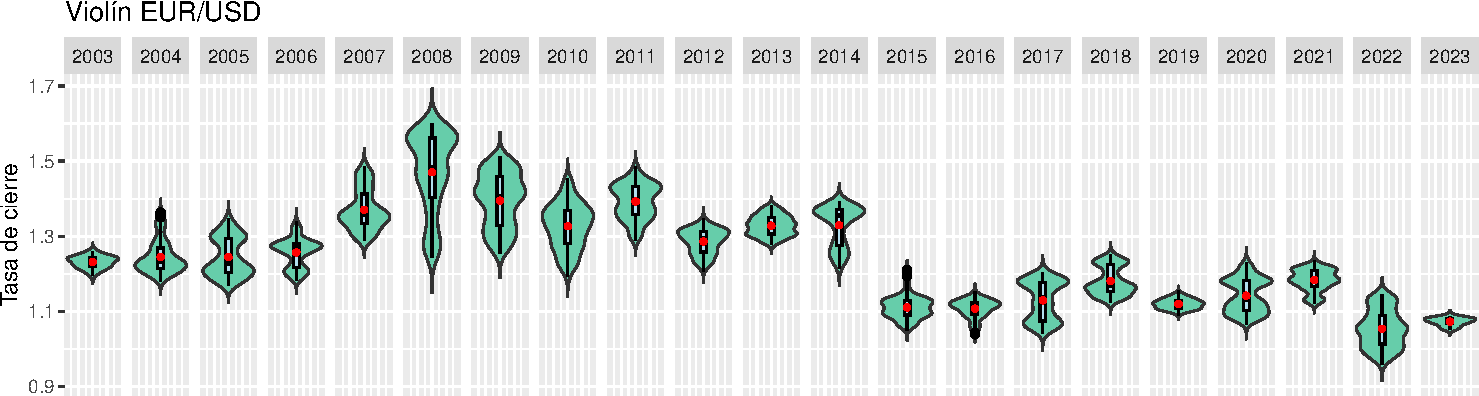
\includegraphics{est1+descriptiva_files/figure-latex/unnamed-chunk-18-1} \end{center}

Una vez obtenido el gráfico, podemos comparar las dispersiones de los datos en cada uno de los años. En específico, se aprecia que la dispersión está entre 1.1 y 1.3 para la mayoría de los años, a excepción del periodo 2007 - 2014, el cual, refleja valores superiores a este rango.

\textbf{Ejercicio:}

\begin{enumerate}
\def\labelenumi{\arabic{enumi}.}
\tightlist
\item
  Utilizando las variables \textbf{Low} y \textbf{Open} de la base de datos de la unidad, elabore un gráfico violín incluyendo un gráfico de caja y el promedio para cada una, diferencia por año. Compara e interprete cada variable por separado.
\end{enumerate}

\hypertarget{barras}{%
\subsection{Barras}\label{barras}}

Una gráfico de barras, es una gráfica para representar los datos cualitativos de una distribución de frecuencia. El procedimiento de construcción es el siguiente \citep[página 29]{anderson}:

\begin{enumerate}
\def\labelenumi{\arabic{enumi}.}
\tightlist
\item
  En uno de los ejes de la gráfica (por lo general en el horizontal).
\item
  Se especifican las etiquetas empleadas para las clases (categorías).
\item
  Para el otro eje de la gráfica (el vertical) se usa una escala para frecuencia, frecuencia relativa o frecuencia porcentual.
\item
  Finalmente, se emplea un ancho de barra fijo y se dibuja sobre cada etiqueta de las clases una barra que se extiende hasta la frecuencia de la clase (a diferencia del histograma, las barras deben estar separadas notoriamente).
\end{enumerate}

Para generar un gráfico de barras en R a partir de un conjunto de datos, se utiliza el siguiente código:

\begin{Shaded}
\begin{Highlighting}[]
\CommentTok{\# Nueva variable para dicotomizar la tasa de cierre del EUR/USD}
\NormalTok{datos}\SpecialCharTok{$}\NormalTok{Close2 }\OtherTok{=} \FunctionTok{ifelse}\NormalTok{(datos}\SpecialCharTok{$}\NormalTok{Close }\SpecialCharTok{\textgreater{}} \FloatTok{1.1}\NormalTok{, }\CommentTok{\# Criterio}
                      \StringTok{"Mayor a 1.1"}\NormalTok{, }\CommentTok{\# Valor asignado si se cumple el criterio}
                      \StringTok{"Menor a  1.1"}\NormalTok{) }\CommentTok{\# Valor asignado si no se cumple el criterio}
\FunctionTok{ggplot}\NormalTok{( }\CommentTok{\# Ambiente gráfico}
  \AttributeTok{data =}\NormalTok{ datos, }\CommentTok{\# Base de datos a utilizar}
  \FunctionTok{aes}\NormalTok{( }\CommentTok{\# Comandos estéticos}
    \AttributeTok{x =}\NormalTok{ Close2)) }\SpecialCharTok{+} \CommentTok{\# Eje Y y variable asociada}
  \FunctionTok{geom\_bar}\NormalTok{( }\CommentTok{\# Objeto a graficar: gráfico de barras}
    \AttributeTok{fill =} \StringTok{"darkgreen"}\NormalTok{) }\SpecialCharTok{+} \CommentTok{\# Color de relleno}
  \FunctionTok{labs}\NormalTok{( }\CommentTok{\# Títulos}
    \AttributeTok{title =} \StringTok{"Barras EUR/USD"}\NormalTok{, }\CommentTok{\# Título del gráfico}
    \AttributeTok{x =} \StringTok{"Tasa de cierre"}\NormalTok{, }\CommentTok{\# Título del eje X}
    \AttributeTok{y =} \StringTok{"Frecuencia"}\NormalTok{) }\CommentTok{\# Título del eje Y}
\end{Highlighting}
\end{Shaded}

\begin{center}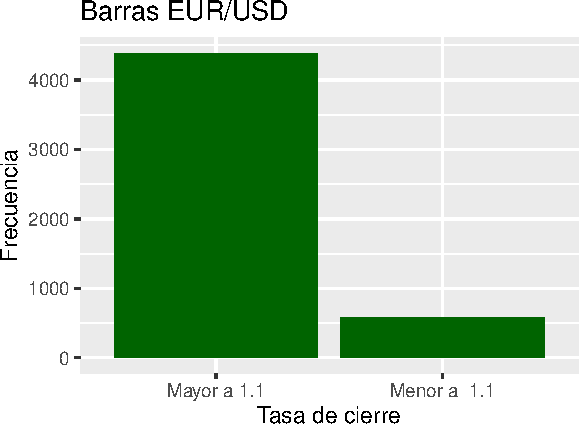
\includegraphics{est1+descriptiva_files/figure-latex/unnamed-chunk-19-1} \end{center}

\textbf{Ejercicio:}

\begin{enumerate}
\def\labelenumi{\arabic{enumi}.}
\tightlist
\item
  Utilizando las variables \textbf{High} y \textbf{Open} de la base de datos de la unidad, elabore un gráfico de barras para cada una. Interprete.
\end{enumerate}

\hypertarget{dispersiuxf3n}{%
\subsection{Dispersión}\label{dispersiuxf3n}}

El gráfico de dispersión es útil para estudiar la relación entre dos variables continuas. Muestra cómo varía un variable en función de la otra y puede ayudar a identificar patrones y tendencias \citep{rowlingson2016data}.

Los pasos para elaborar un gráfico de caja son los siguiente \citep{healy2019data}:

\begin{enumerate}
\def\labelenumi{\arabic{enumi}.}
\tightlist
\item
  Elegir dos variables continuas de la base de datos a trabajar. Cada fila corresponde a una observación, por lo cual, hay una correspondencia entre los valores de una misma fila.
\item
  Elegir la variable estará en el eje X y Y.
\item
  Representar cada par ordenado con un punto.
\end{enumerate}

Para generar un gráfico de dispersión en R a partir de un conjunto de datos, se utiliza el siguiente código:

\begin{Shaded}
\begin{Highlighting}[]
\FunctionTok{ggplot}\NormalTok{( }\CommentTok{\# Ambiente gráfico}
  \AttributeTok{data =}\NormalTok{ datos, }\CommentTok{\# Base de datos a utilizar}
  \FunctionTok{aes}\NormalTok{( }\CommentTok{\# Comando estéticos}
    \AttributeTok{x =}\NormalTok{ Open, }\CommentTok{\# Eje X y variable asociada}
    \AttributeTok{y =}\NormalTok{ Close)) }\SpecialCharTok{+} \CommentTok{\# Eje Y y variable asociada}
  \FunctionTok{geom\_point}\NormalTok{( }\CommentTok{\# Objeto a graficar: Gráfico de dispersión}
    \AttributeTok{color =} \StringTok{"darkblue"}\NormalTok{, }\CommentTok{\# Color}
    \AttributeTok{alpha =} \FloatTok{0.3}\NormalTok{) }\SpecialCharTok{+} \CommentTok{\# Opacidad}
  \FunctionTok{labs}\NormalTok{( }\CommentTok{\# Títulos}
    \AttributeTok{title =} \StringTok{"Tasa de apertura y cierre del EUR/USD"}\NormalTok{, }\CommentTok{\# Título del gráfico}
    \AttributeTok{x =} \StringTok{"Tasa de apertura"}\NormalTok{, }\CommentTok{\# Título del eje X}
    \AttributeTok{y =} \StringTok{"Tasa de cierre"}\NormalTok{) }\CommentTok{\# Título del eje Y}
\end{Highlighting}
\end{Shaded}

\begin{center}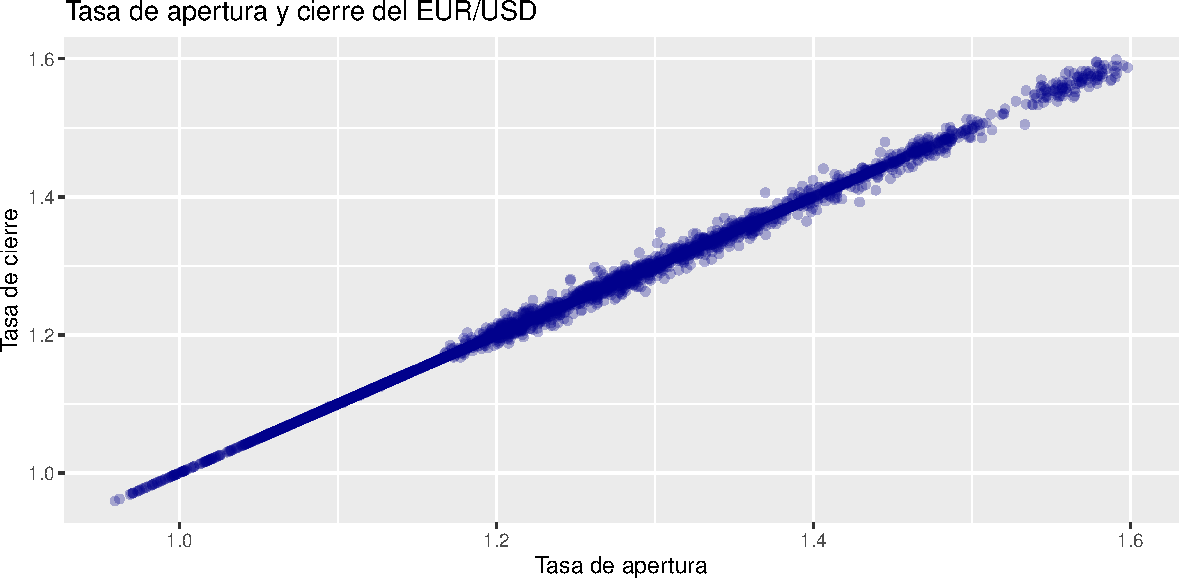
\includegraphics{est1+descriptiva_files/figure-latex/unnamed-chunk-20-1} \end{center}

\textbf{Ejercicio:}

\begin{enumerate}
\def\labelenumi{\arabic{enumi}.}
\tightlist
\item
  Utilizando las variables \textbf{High} y \textbf{Low} de la base de datos de la unidad, elabore un gráfico de dispersión. Interprete.
\end{enumerate}

\textbf{Ejemplo:}

\begin{enumerate}
\def\labelenumi{\arabic{enumi}.}
\tightlist
\item
  Es posible utilizar el gráfico de dispersión con variables que en su naturaleza son discretas. En este sentido, elabore un gráfico de dispersión entre el año de medición y el valor promedio de tasa de apertura del EUR/USD (guarde el gráfico en una variable).
\end{enumerate}

\begin{Shaded}
\begin{Highlighting}[]
\NormalTok{g }\OtherTok{=} \FunctionTok{ggplot}\NormalTok{( }\CommentTok{\# Ambiente gráfico}
  \AttributeTok{data =}\NormalTok{ datos, }\CommentTok{\# Base de datos a utilizar}
  \FunctionTok{aes}\NormalTok{( }\CommentTok{\# Comando estéticos}
    \AttributeTok{x =}\NormalTok{ Ano, }\CommentTok{\# Eje X y variable asociada}
    \AttributeTok{y =}\NormalTok{ Open, }\CommentTok{\# Eje Y y variable asociada}
    \AttributeTok{group =} \DecValTok{1}\NormalTok{)) }\SpecialCharTok{+} \CommentTok{\# Comando únicamente necesario para la pregunta 2}
  \FunctionTok{geom\_point}\NormalTok{( }\CommentTok{\# Objeto a graficar}
    \AttributeTok{stat =} \StringTok{"summary"}\NormalTok{, }\CommentTok{\# Tipo de información a graficar: resumen}
    \AttributeTok{fun =} \StringTok{"mean"}\NormalTok{) }\SpecialCharTok{+} \CommentTok{\# Tipo de resumen: promedio de la variable Y}
  \FunctionTok{labs}\NormalTok{( }\CommentTok{\# Títulos}
    \AttributeTok{title =} \StringTok{"Tasa de apertura promedio del EUR/USD por año"}\NormalTok{, }\CommentTok{\# Título del gráfico}
    \AttributeTok{x =} \StringTok{"Año"}\NormalTok{, }\CommentTok{\# Título del eje X}
    \AttributeTok{y =} \StringTok{"Tasa de apertura"}\NormalTok{) }\CommentTok{\# Título del eje Y}
\NormalTok{g }\CommentTok{\# Desplegamos el gráfico guardado}
\end{Highlighting}
\end{Shaded}

\begin{center}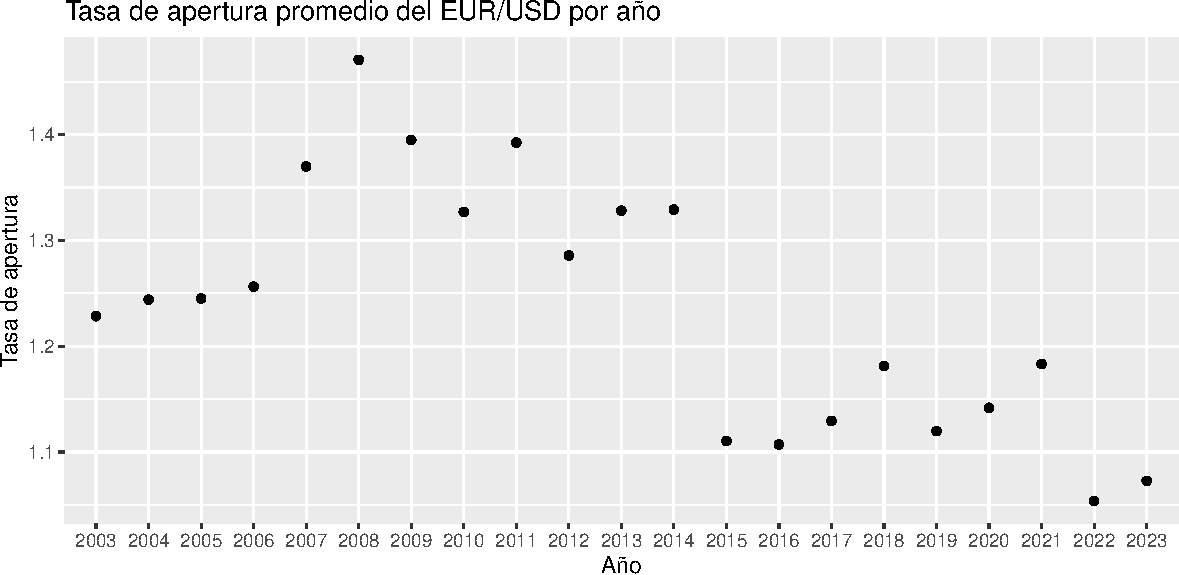
\includegraphics{est1+descriptiva_files/figure-latex/unnamed-chunk-21-1} \end{center}

\begin{enumerate}
\def\labelenumi{\arabic{enumi}.}
\setcounter{enumi}{1}
\tightlist
\item
  Añadir al gráfico un formato de líneas entre los puntos. Interprete.
\end{enumerate}

\begin{Shaded}
\begin{Highlighting}[]
\NormalTok{g }\OtherTok{=}\NormalTok{ g }\SpecialCharTok{+} \CommentTok{\# Añadimos otro gráfico}
  \FunctionTok{geom\_line}\NormalTok{( }\CommentTok{\# Objeto a graficar: lineas}
    \AttributeTok{stat =} \StringTok{"summary"}\NormalTok{, }\CommentTok{\# Tipo de información a graficar: resumen}
    \AttributeTok{fun =} \StringTok{"mean"}\NormalTok{) }\CommentTok{\# Tipo de resumen: promedio de la variable Y}
\NormalTok{g }\CommentTok{\# Desplegamos el gráfico guardado}
\end{Highlighting}
\end{Shaded}

\begin{center}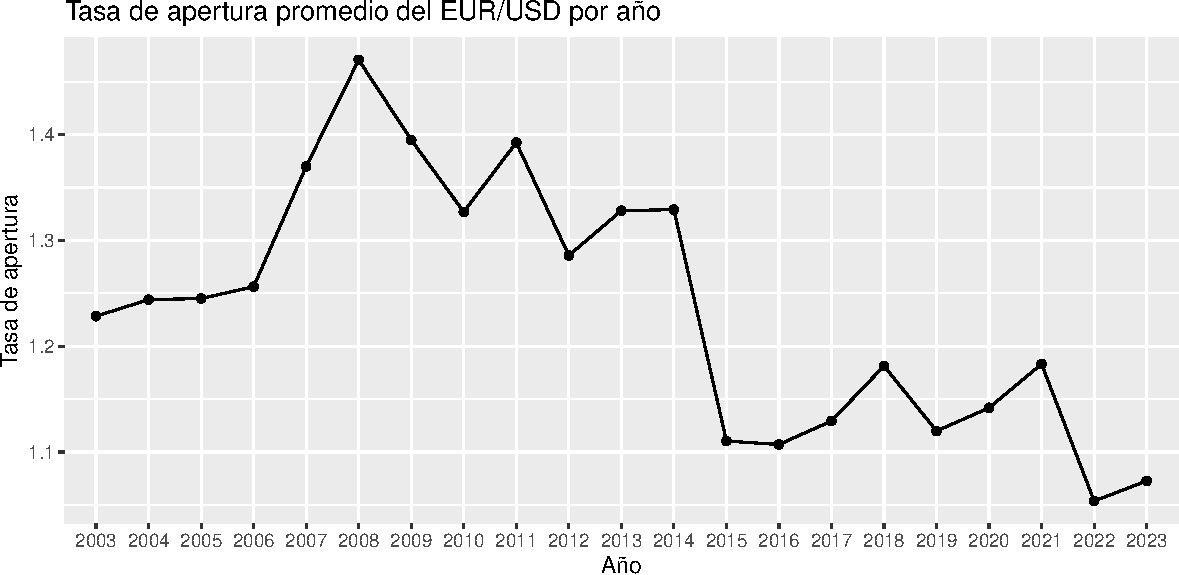
\includegraphics{est1+descriptiva_files/figure-latex/unnamed-chunk-22-1} \end{center}

Hasta el 2008 la tasa promedio de apertura estuvo en alza, posteriormente, la tasa decayó a un valor inferior a 1.2.

\begin{enumerate}
\def\labelenumi{\arabic{enumi}.}
\setcounter{enumi}{2}
\tightlist
\item
  Grafique el valor de la tasa de apertura del EUR/USD desde el 2020 hasta el 2022 separadamente. Interprete.
\end{enumerate}

\begin{Shaded}
\begin{Highlighting}[]
\NormalTok{datos}\SpecialCharTok{$}\NormalTok{Date }\OtherTok{=} \FunctionTok{as.Date}\NormalTok{(datos}\SpecialCharTok{$}\NormalTok{Date) }\CommentTok{\# Fechas en formato fecha de R}
\NormalTok{g }\OtherTok{=} \FunctionTok{ggplot}\NormalTok{( }\CommentTok{\# Ambiente gráfico}
  \AttributeTok{data =}\NormalTok{ datos[datos}\SpecialCharTok{$}\NormalTok{Ano }\SpecialCharTok{\%in\%} \DecValTok{2020}\SpecialCharTok{:}\DecValTok{2022}\NormalTok{,], }\CommentTok{\# Datos de los años 2020 al 2022}
  \FunctionTok{aes}\NormalTok{( }\CommentTok{\# Comando estéticos}
    \AttributeTok{x =}\NormalTok{ Date, }\CommentTok{\# Comandos estéticos: Eje X y variable asociada}
    \AttributeTok{y =}\NormalTok{ Open)) }\SpecialCharTok{+} \CommentTok{\# Eje Y y variable asociada}
  \FunctionTok{geom\_point}\NormalTok{( }\CommentTok{\# Objeto a graficar}
    \AttributeTok{alpha =} \FloatTok{0.5}\NormalTok{, }\CommentTok{\# Opacidad}
    \AttributeTok{size =} \FloatTok{0.6}\NormalTok{) }\SpecialCharTok{+} \CommentTok{\# Tamaño}
  \FunctionTok{theme}\NormalTok{( }\CommentTok{\# Aspectos visuales del gráfico}
    \AttributeTok{axis.text.x =} \FunctionTok{element\_blank}\NormalTok{()) }\SpecialCharTok{+} \CommentTok{\# Eliminamos el texto del eje X}
  \FunctionTok{facet\_wrap}\NormalTok{( }\CommentTok{\# Segregación del gráfico}
    \FunctionTok{vars}\NormalTok{(Ano), }\CommentTok{\# Variable que se utiliza para segregar el gráfico}
    \AttributeTok{nrow =} \DecValTok{1}\NormalTok{, }\CommentTok{\# Disposición visual: una fila}
    \AttributeTok{scales =} \StringTok{"free\_x"}\NormalTok{) }\SpecialCharTok{+} \CommentTok{\# La escala del eje X es independiente para gráfico}
  \FunctionTok{labs}\NormalTok{( }\CommentTok{\# Títulos}
    \AttributeTok{title =} \StringTok{"Tasa de apertura del EUR/USD desde el 2020 hasta el 2022"}\NormalTok{, }\CommentTok{\# Título del gráfico}
    \AttributeTok{x =} \StringTok{"Fecha"}\NormalTok{, }\CommentTok{\# Título del eje X}
    \AttributeTok{y =} \StringTok{"Tasa de apertura"}\NormalTok{) }\CommentTok{\# Título del eje Y}
\NormalTok{g }\CommentTok{\# Desplegamos el gráfico guardado}
\end{Highlighting}
\end{Shaded}

\begin{center}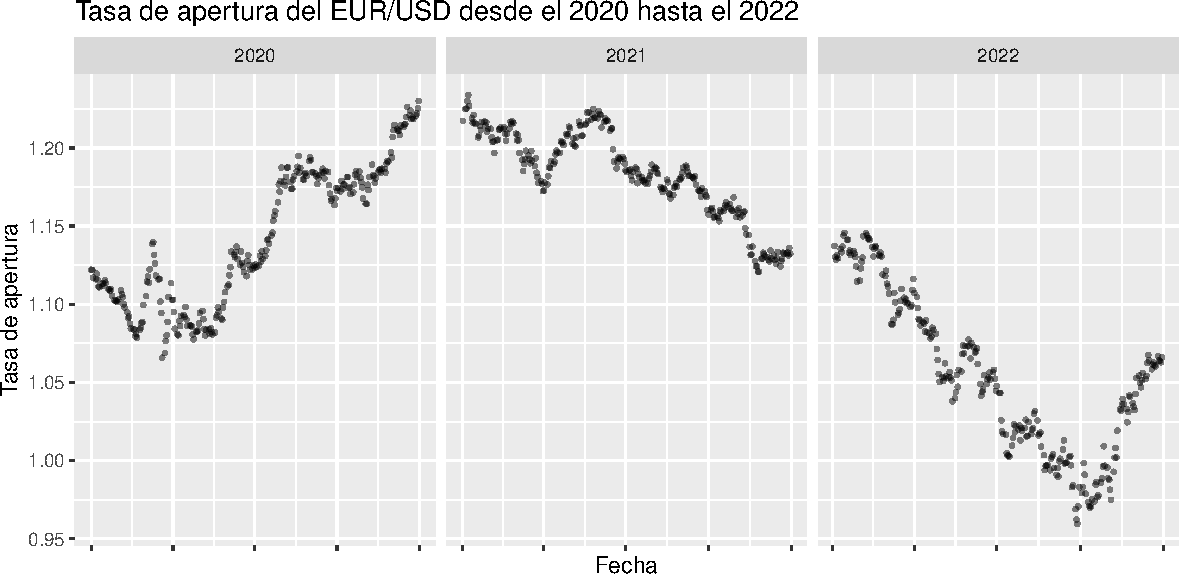
\includegraphics{est1+descriptiva_files/figure-latex/unnamed-chunk-23-1} \end{center}

Durante los 3 años consecutivos, se observa que únicamente en el 2020 la tendencia de la tasa de apertura es al alza, mientra que para los otros dos años hubo un decaimiento en el valor de esta.

\begin{enumerate}
\def\labelenumi{\arabic{enumi}.}
\setcounter{enumi}{3}
\tightlist
\item
  Grafique el valor de la tasa de apertura del EUR/USD diferenciando por año. Interprete.
\end{enumerate}

\begin{Shaded}
\begin{Highlighting}[]
\NormalTok{g }\OtherTok{=} \FunctionTok{ggplot}\NormalTok{( }\CommentTok{\# Ambiente gráfico}
  \AttributeTok{data =}\NormalTok{ datos, }\CommentTok{\# Base de datos a utilizar}
  \FunctionTok{aes}\NormalTok{( }\CommentTok{\# Comando estéticos}
    \AttributeTok{x =}\NormalTok{ Date, }\CommentTok{\# Comandos estéticos: Eje X y variable asociada}
    \AttributeTok{y =}\NormalTok{ Open, }\CommentTok{\# Eje Y y variable asociada}
    \AttributeTok{color =}\NormalTok{ Ano)) }\SpecialCharTok{+} \CommentTok{\# Color según el año}
  \FunctionTok{geom\_point}\NormalTok{( }\CommentTok{\# Objeto a graficar}
    \AttributeTok{alpha =} \FloatTok{0.5}\NormalTok{, }\CommentTok{\# Opacidad}
    \AttributeTok{size =} \FloatTok{0.7}\NormalTok{) }\SpecialCharTok{+} \CommentTok{\# Tamaño}
  \FunctionTok{labs}\NormalTok{( }\CommentTok{\# Títulos}
    \AttributeTok{color =} \StringTok{"Año"}\NormalTok{, }\CommentTok{\# Título de la leyenda}
    \AttributeTok{title =} \StringTok{"Tasa de apertura del EUR/USD"}\NormalTok{, }\CommentTok{\# Título del gráfico}
    \AttributeTok{x =} \StringTok{"Fecha"}\NormalTok{, }\CommentTok{\# Título del eje X}
    \AttributeTok{y =} \StringTok{"Tasa de apertura"}\NormalTok{) }\SpecialCharTok{+} \CommentTok{\# Título del eje Y}
  \FunctionTok{guides}\NormalTok{( }\CommentTok{\# Edición de escalas}
    \AttributeTok{color =} \FunctionTok{guide\_legend}\NormalTok{( }\CommentTok{\# Escala de color de la leyenda}
      \AttributeTok{override.aes =} \FunctionTok{list}\NormalTok{( }\CommentTok{\# Comando estéticos asociados}
        \AttributeTok{alpha =} \DecValTok{1}\NormalTok{, }\CommentTok{\# Opacidad de los puntos}
        \AttributeTok{size =} \DecValTok{3}\NormalTok{))) }\CommentTok{\# Tamaño de los puntos}
\NormalTok{g }\CommentTok{\# Desplegamos el gráfico guardado}
\end{Highlighting}
\end{Shaded}

\begin{center}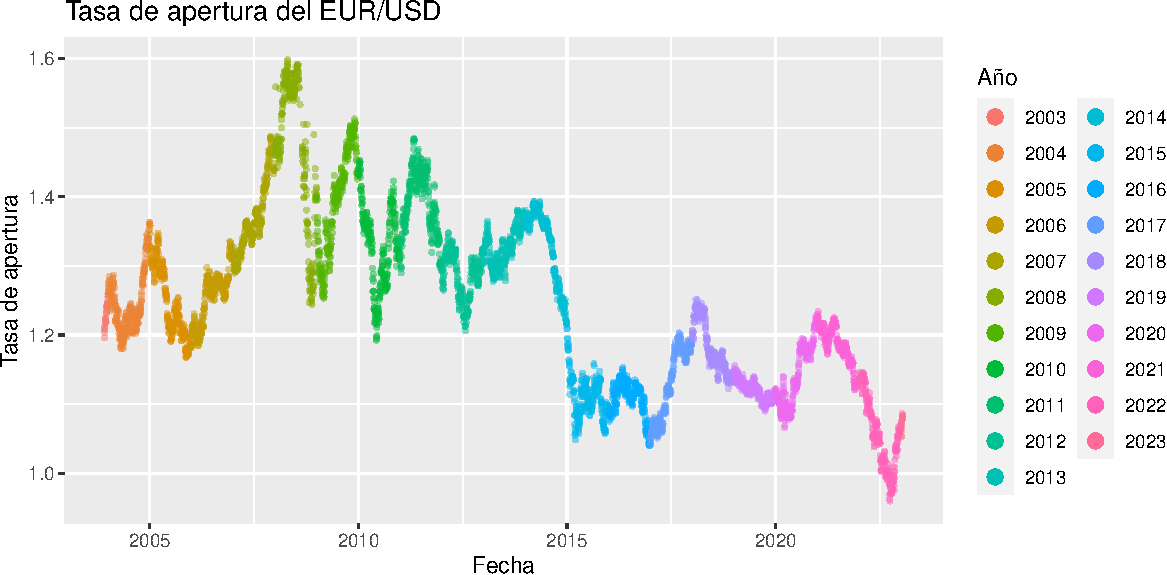
\includegraphics{est1+descriptiva_files/figure-latex/unnamed-chunk-24-1} \end{center}

Al observar la evolución histórica de la tasa de apertura diferenciada por año, se aprecia que el periodo 2008 - 2010 es aquel con predominancia de valores más altos. Por otro lado, desde el 2016, se registraron pro primera vez valores menores a 1.1. En años posteriores, no ha observado que la tasa supere los 1.3 puntos.

\begin{enumerate}
\def\labelenumi{\arabic{enumi}.}
\setcounter{enumi}{4}
\tightlist
\item
  Grafique el valor el valor promedio de la tasa más alta versus la más baja del EUR/USD para cada uno de los años. Interprete.
\end{enumerate}

\begin{Shaded}
\begin{Highlighting}[]
\NormalTok{g }\OtherTok{=} \FunctionTok{ggplot}\NormalTok{( }\CommentTok{\# Ambiente gráfico}
  \AttributeTok{data =} \FunctionTok{aggregate}\NormalTok{( }\CommentTok{\# Función para resumir una base de datos (crea una nueva base)}
    \AttributeTok{x =}\NormalTok{ datos, }\CommentTok{\# Indicar la base de datos a modificar}
    \AttributeTok{by =} \FunctionTok{list}\NormalTok{(Año }\OtherTok{=}\NormalTok{ datos}\SpecialCharTok{$}\NormalTok{Ano), }\CommentTok{\# Variable por la cual se genera el resumen, y nombre asignado}
    \AttributeTok{FUN =}\NormalTok{ mean), }\CommentTok{\# Resumen que se genera en las columnas de la base de datos}
  \FunctionTok{aes}\NormalTok{( }\CommentTok{\# Comandos estéticos}
    \AttributeTok{x =}\NormalTok{ Low, }\CommentTok{\# Eje X y variable asociada}
    \AttributeTok{y =}\NormalTok{ High, }\CommentTok{\# Eje Y y variable asociada}
    \AttributeTok{color =}\NormalTok{ Año)) }\SpecialCharTok{+} \CommentTok{\# Color según variable}
  \FunctionTok{geom\_point}\NormalTok{() }\SpecialCharTok{+} \CommentTok{\# Objeto a graficar: gráfico de dispersión}
  \FunctionTok{labs}\NormalTok{( }\CommentTok{\# Títulos}
    \AttributeTok{title =} \StringTok{"Promedio de la tasa más alta y más baja del EUR/USD"}\NormalTok{, }\CommentTok{\# Título del gráfico}
    \AttributeTok{x =} \StringTok{"Tasa más baja"}\NormalTok{, }\CommentTok{\# Título el eje X}
    \AttributeTok{y =} \StringTok{"Tasa más alta"} \CommentTok{\# Título el eje Y}
\NormalTok{  )}
\NormalTok{g }\CommentTok{\# Desplegamos el gráfico guardado}
\end{Highlighting}
\end{Shaded}

\begin{center}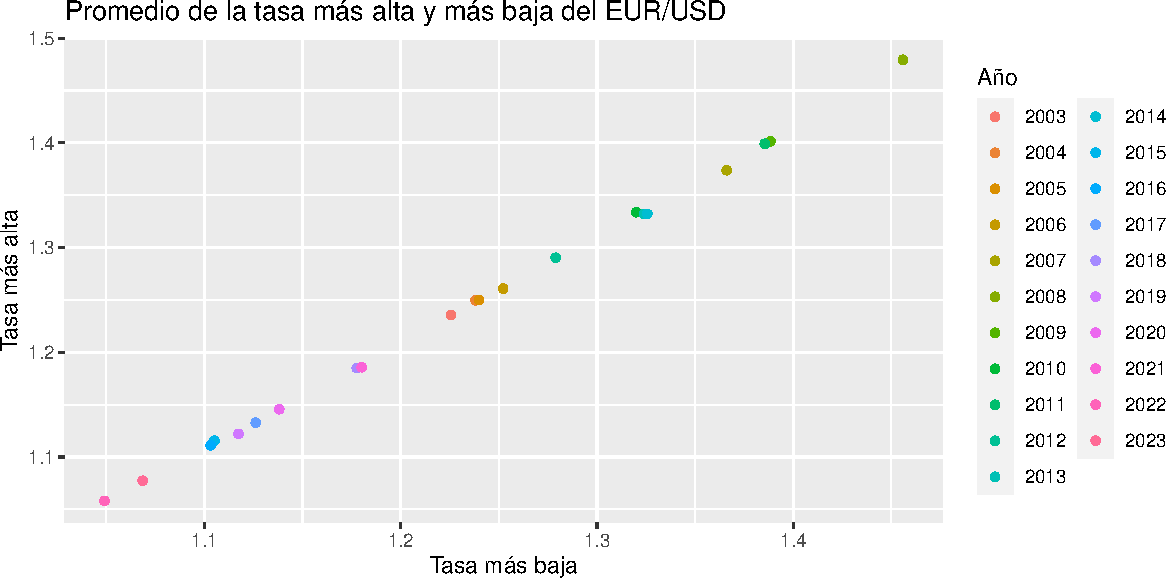
\includegraphics{est1+descriptiva_files/figure-latex/unnamed-chunk-25-1} \end{center}

El gráfico da cuenta de una tendencia positiva entre la tasa promedio más baja y más alta registrada en los diversos años, siendo el año 2018 aquel que destaca con las tasas promedio más altas.

\textbf{Ejercicio:}

\begin{enumerate}
\def\labelenumi{\arabic{enumi}.}
\tightlist
\item
  Elabore un gráfico de dispersión entre el año de medición y el valor promedio de tasa de cierre del EUR/USD (guarde el gráfico en una variable).
\item
  Añadir al gráfico un formato de líneas entre los puntos. Interprete.
\item
  Grafique el valor de la tasa de cierre del EUR/USD desde el 2010 hasta el 2013 separadamente. Interprete.
\item
  Grafique el valor de la tasa de cierre del EUR/USD diferenciando por año. Interprete.
\item
  Grafique el valor el valor promedio de la tasa de cierre versus la más baja del EUR/USD para cada uno de los años. Interprete.
\end{enumerate}

\hypertarget{probabilidad-y-variables-aleatorias.}{%
\chapter{Probabilidad y variables aleatorias.}\label{probabilidad-y-variables-aleatorias.}}

\hypertarget{elementos-de-probabilidad}{%
\section{Elementos de probabilidad}\label{elementos-de-probabilidad}}

\hypertarget{espacio-muestral}{%
\subsection{Espacio muestral}\label{espacio-muestral}}

\hypertarget{funciuxf3n-de-probabilidad}{%
\subsection{Función de probabilidad}\label{funciuxf3n-de-probabilidad}}

\hypertarget{variable-aleatoria}{%
\section{Variable aleatoria}\label{variable-aleatoria}}

\hypertarget{funciuxf3n-de-probabilidad-1}{%
\subsection{Función de probabilidad}\label{funciuxf3n-de-probabilidad-1}}

\hypertarget{funciuxf3n-de-distribuciuxf3n}{%
\subsection{Función de distribución}\label{funciuxf3n-de-distribuciuxf3n}}

\hypertarget{variable-aleatoria-discreta}{%
\section{Variable aleatoria discreta}\label{variable-aleatoria-discreta}}

\hypertarget{uniforme}{%
\subsection{Uniforme}\label{uniforme}}

\hypertarget{bernoulli}{%
\subsection{Bernoulli}\label{bernoulli}}

\hypertarget{binomial}{%
\subsection{Binomial}\label{binomial}}

\hypertarget{poisson}{%
\subsection{Poisson}\label{poisson}}

\hypertarget{variable-aleatoria-continua}{%
\section{Variable aleatoria continua}\label{variable-aleatoria-continua}}

\hypertarget{uniforme-1}{%
\subsection{Uniforme}\label{uniforme-1}}

\hypertarget{exponencial}{%
\subsection{Exponencial}\label{exponencial}}

\hypertarget{normal}{%
\subsection{Normal}\label{normal}}

\hypertarget{t---student}{%
\subsection{T - Student}\label{t---student}}

\hypertarget{ji---cuadrado}{%
\subsection{Ji - Cuadrado}\label{ji---cuadrado}}

\hypertarget{esperanza}{%
\section{Esperanza}\label{esperanza}}

\hypertarget{variable-aleatoria-discreta-1}{%
\subsection{Variable aleatoria discreta}\label{variable-aleatoria-discreta-1}}

\hypertarget{variable-aleatoria-continua-1}{%
\subsection{Variable aleatoria continua}\label{variable-aleatoria-continua-1}}

\hypertarget{varianza}{%
\section{Varianza}\label{varianza}}

\hypertarget{variable-aleatoria-discreta-2}{%
\subsection{Variable aleatoria discreta}\label{variable-aleatoria-discreta-2}}

\hypertarget{variable-aleatoria-continua-2}{%
\subsection{Variable aleatoria continua}\label{variable-aleatoria-continua-2}}

\hypertarget{distribuciones-muestrales-y-pruebas-de-hipuxf3tesis}{%
\chapter{Distribuciones muestrales y pruebas de hipótesis}\label{distribuciones-muestrales-y-pruebas-de-hipuxf3tesis}}

\hypertarget{distribuciuxf3n-de-muestreo-de-la-media}{%
\section{Distribución de muestreo de la media}\label{distribuciuxf3n-de-muestreo-de-la-media}}

\hypertarget{estandarizaciuxf3n}{%
\subsection{Estandarización}\label{estandarizaciuxf3n}}

\hypertarget{distribuciuxf3n-de-la-media}{%
\subsection{Distribución de la media}\label{distribuciuxf3n-de-la-media}}

\hypertarget{teorema-del-luxedmite-central}{%
\subsection{Teorema del límite central}\label{teorema-del-luxedmite-central}}

\hypertarget{distribuciuxf3n-de-muestreo-de-la-varianza}{%
\section{Distribución de muestreo de la varianza}\label{distribuciuxf3n-de-muestreo-de-la-varianza}}

\hypertarget{la-distribuciuxf3n-t-student}{%
\section{La distribución T-Student}\label{la-distribuciuxf3n-t-student}}

\hypertarget{prueba}{%
\section{Pruebas de hipótesis}\label{prueba}}

\hypertarget{una-media}{%
\subsection{Una media}\label{una-media}}

\hypertarget{diferencia-de-medias}{%
\subsection{Diferencia de medias}\label{diferencia-de-medias}}

\hypertarget{comparaciuxf3n-de-varianzas}{%
\subsection{Comparación de varianzas}\label{comparaciuxf3n-de-varianzas}}

\hypertarget{diferencia-de-proporciones}{%
\subsection{Diferencia de proporciones}\label{diferencia-de-proporciones}}

\hypertarget{intervalos-de-confianza}{%
\chapter{Intervalos de confianza}\label{intervalos-de-confianza}}

\hypertarget{una-media-1}{%
\section{Una media}\label{una-media-1}}

\hypertarget{bajo-distribuciuxf3n-normal}{%
\subsection{Bajo distribución normal}\label{bajo-distribuciuxf3n-normal}}

\hypertarget{asintuxf3tico}{%
\subsection{Asintótico}\label{asintuxf3tico}}

\hypertarget{diferencia-de-medias-1}{%
\section{Diferencia de medias}\label{diferencia-de-medias-1}}

\hypertarget{compraraciuxf3n-de-varianzas}{%
\section{Compraración de varianzas}\label{compraraciuxf3n-de-varianzas}}

\hypertarget{diferencia-de-proporciones-1}{%
\section{Diferencia de proporciones}\label{diferencia-de-proporciones-1}}

  \bibliography{refs.bib}

\end{document}
